\documentclass[11pt]{article}

\usepackage[top=50mm, bottom=50mm, left=50mm, right=50mm]{geometry}
%\usepackage[a4paper,top=2.5cm,bottom=2.5cm,left=2.5cm,right=2.5cm,marginparwidth=1.75cm]{geometry}
% for adding numbers for lines 
\usepackage{lineno}
\usepackage{amssymb}
\usepackage{amsmath}
\usepackage{amsthm}
\usepackage{epsfig}
\usepackage{caption}
\usepackage{subcaption}
\usepackage{graphics}
\usepackage{graphicx}
\usepackage{multirow}
\usepackage{multicol}
\usepackage{float}
\usepackage{multirow}
\usepackage{color}
\usepackage{lineno}
\usepackage{fullpage}
\usepackage{hyperref}
\usepackage[normalem]{ulem} 
\usepackage{makeidx}
\usepackage{xspace}
\usepackage{wrapfig}
\usepackage{newfloat}
\makeindex

\DeclareFloatingEnvironment[name={Supplementary Figure},fileext=lof]{suppfigure}


\newtheorem{theorem}{Theorem}
\newtheorem{Definition}{Definition}
\newtheorem{corollary}{Corollary}
\newtheorem{Theorem}{Theorem}
\newtheorem{Lemma}{Lemma}
\newtheorem{Claim}{Claim}
\newtheorem{Notation}{Notation}
\newtheorem{Algorithm}{Algorithm}
\newtheorem{Observation}{Observation}


%%%%%%%%%%%%%%% macros by yusu %%%%%%%%%%%%%
\newtheorem{lemma}{Lemma}
\newtheorem{claim}{Claim}
\newtheorem{obs}{Observation}

\definecolor{darkred}{rgb}{1, 0.1, 0.3}
\definecolor{darkblue}{rgb}{0.1, 0.1, 1}
\definecolor{darkgreen}{rgb}{0,0.6,0.5}
\newcommand{\yusu}[1]		{{ \textcolor{darkblue} {{\sc Yusu Says:} #1}}}

\newcommand {\mm}[1] {\ifmmode{#1}\else{\mbox{\(#1\)}}\fi}
\newcommand{\denselist}{\itemsep 0pt\parsep=1pt\partopsep 0pt}

\newcommand{\etal}		{{et al.}\xspace}
\newcommand{\myeg}	{{e.g.}\xspace}

\newcommand{\eps}		{\varepsilon}
\newcommand{\myanceq}	{{\succeq}} %ancerster 
\newcommand{\myanc}	{{\succ}} %ancerster 
\newcommand{\mydesceq} {{\preceq}}
\newcommand{\mydesc}		{{\prec}}
\newcommand{\dgh}		{\delta_{\mathcal{GH}}} %GH distance
\newcommand{\optdI}	{\mu}
\newcommand{\myeps}	{\eps}
\newcommand{\mygood}		{{good}\xspace}
\newcommand{\myk}		{\tau} %{\kappa}
\newcommand{\mydelta}	{\delta}
\newcommand{\nTone}	{{\widehat{T}_{1, \mydelta}^{\hat{f}}}}
\newcommand{\nTtwo}	{{\widehat{T}_{2, \mydelta}^{\hat{g}}}}
\newcommand{\Img}		{{\mathrm{Im}}}
\newcommand{\myL}		{{L}}
\newcommand{\superlevel}		{{super-level}\xspace}
\newcommand{\myC}		{{\mathrm{C}}}
\newcommand{\setSL}	{{\mathcal{L}}}
\newcommand{\slone}[1] 	{{\mathrm{L}^{(1)}_{#1}}}
\newcommand{\sltwo}[1] 	{{\mathrm{L}^{(2)}_{#1}}}
\newcommand{\hatT}		{{\widehat{T}}}
\newcommand{\levelC}		{\mathrm{Ch}} %{{levelC}}
\newcommand{\LCA}		{{LCA}}%common ancester
\newcommand{\DPalg}	{{\sf DPgoodmap}}
\newcommand{\modifyDPalg}	{{\sf modified-DP}}
\newcommand{\myF}		{{\mathcal{F}}}
\newcommand{\mypartial}[1]		{{partial-{#1}-good}\xspace}
\newcommand{\myvalue}		{\mathrm{value}}
\newcommand{\degbound}		{{degree-bound}\xspace}
\newcommand{\mydepth}		{{depth}\xspace}
\newcommand{\ep}		{{\varepsilon_p}}

\newcommand{\Intdopt}		{{\mydelta^*}}
\newcommand{\criSet}		{{\Pi}}
\newcommand{\Tcal}			{\mathcal{T}}
\newcommand{\mycost}		{{\mathrm{cost}}}
\newcommand{\uTone}		{{|T_1^f|}}
\newcommand{\uTwo}		{{|T_2^g|}}
\newcommand{\uT}				{{|T|}}
\newcommand{\mywF}		{{w^F}}
\newcommand{\mykpara}	{{\myk_\mydelta}}
\newcommand{\newdepth}	{{depth}}
\newcommand{\newtau}	{{\widehat{\tau}}}

\newcommand{\sensiblepair}     {{sensible-pair}\xspace}
\newcommand{\Edgelistpair}      {{Edge-list pair}\xspace}
\newcommand{\edgelistpair}      {{edge-list pair}\xspace}
\newcommand{\Fnew}          {{F_{new}}}
\newcommand{\Fold}          {{F_{old}}}

%%%%%%%%%%%%%% macros by yusu end %%%%%%%%%%%%%

\begin{document}

\title{Monitoring Health Systems by Estimating Excess Mortality}
 
\author{
{Rolando J. Acosta \footnote{Department of Biostatistics, Harvard University, Cambridge, MA, USA}} \and {Rafael A. Irizarry \footnote{Department of Data Science, Dana-Farber Cancer Institute; \newline Department of Biostatistics, Harvard University, Cambridge, MA, USA}}
}

%\begin{document}
\maketitle
%\linenumbers
\setcounter{page}{0}

\begin{abstract}
Monitoring health systems during and after natural disasters, epidemics, or outbreaks is paramount to guiding policy decisions and interventions. In the case of natural disaster the effects of these events on public health can be \textit{direct} or \textit{indirect}. Direct effects are defined as those resulting from the immediate destruction such as drowning and trauma from flying debris, while indirect effects are delayed, longer lasting, and, often, harder to measure or detect. In the case of outbreaks and epidemics, lack of comprehensive testing or reporting can lead to challenges in measuring direct effects, while indirect effects can arise due to, for example, increased stress levels or reduced access to health services. When the effects are long lasting and difficult to detect, in the short term, the accumulated effects can actually be devastating. Improved access to mortality data provides an opportunity to develop data-driven approaches that can help monitor health systems.
Here we describe a statistical methodology and software that facilitates data-driven approaches. Our work was motivated by events occurring in Puerto Rico after the passage of Hurricane Mar\'ia, but can be applied in other contexts such as estimating the effects of an epidemic in the presence of inaccurate reporting of cases. We make our tools available as a free and open source R package and an interactive webtool.
\end{abstract}

\newpage

\section{Introduction}
\label{sec:introduction}
Hurricane Mar\'ia made landfall in Puerto Rico on September 20, 2017, interrupting the water supply, electricity, telecommunications networks, and access to medical care\cite{updates2018puerto, rogers2017puerto}. Two weeks after the hurricane the official death count stood at 16\cite{hoyos2018puerto}. This figure was in conflict with estimates obtained using a historical approach by groups that ostensibly had access to death counts for September and October from the demographic registry of Puerto Rico, not yet readily available to the general public. By comparing these two numbers to historical averages, additional deaths were estimated to be in excess of 1,000 \cite{santos2018use, robles2017official, rivera2018estimating, pascual2017nearly} raising concerns that Puerto Rico was in the midst of a public health crisis. However, on December 13, 2017, almost three months after landfall, Puerto Rico’s Secretary of the Department of Public Safety, dismissed these concerns \cite{robles2017official}. As of May 2017 the official death count stood at 64 \cite{hoyos2018puerto} and it appeared the government was not concerned. On May 29, 2018 three days after a study was published describing a survey of 3,299 households and reporting a much higher estimate of the death count received worldwide media coverage \cite{kishore2018mortality}, the government finally made the data public and acknowledged the possibility of a higher excess death count of 1,427 \cite{report2019} based on the vital statistics numbers. On August 2018 the official death toll was revised to 2,975 based on a study commissioned by the government of Puerto Rico \cite{santos2018differential}.

More recently, the limited capacity to perform molecular tests has raised concerns that COVID-19 cases are under-reported in several jurisdictions in the United States and across the world. Simultaneously, polls show that a substantial proportion of the US population believes that reported COVID-19 fatalities are inflated \cite{talev2020}. Estimating excess mortality provides a way to measure the impact of the epidemic, even in the presence of inaccurate reporting.

Here we describe data-driven tools that, when applied to death records, can help answer questions such as: are current excess mortality counts reason for concern? For how long is the population affected by an event?  How much do the effects vary across jurisdictions?  Was there a specific demographic that was at greater risk? What type of medical conditions need the most attention? Our approach provide informative summaries that can help detect concerning patterns, including tools can also help detect abnormalities in close to real-time. 

The main goal of our method is to determine if an observed death count, for a given demographic and period of time is \textit{unusually high}. Reporting unusually high death rates can alert government officials and policy makers that an intervention is required. Because of stochastic variation, \textit{usual} cannot be defined with one number and instead a distribution is appropriate. The uncertainty associated with count data, such as daily deaths totals, are typically accounted for with Poisson models \cite{mccullagh19831989, agresti2015foundations}. However, these models do not account for year-to-year increases or decreases that may be due to natural, possibly correlated in time, stochastic variation. Examples of possible causes are variation in the severity of common colds in the winter or the number of extremely hot days in the summer. The engine behind our tools is a statistical model that accounts for such variability and can be fit to data stratified by demographic group or cause of death. 

To demonstrate the utility of our approach, we use it to provide a detailed picture of the effect Hurricane Mar\'ia had on mortality in Puerto Rico and compare these to those observed in Hugo and Georges, two previous hurricanes in Puerto Rico, Katrina in Louisiana, Irma in Florida, and Sandy in New Jersey. We also investigate the effects of the Chikungunya epidemic in Puerto Rico in 2014 and compare it to estimates from the 2020 spring during the COVID-19 pandemic. We also apply our method to recently released state-level data by the CDC and compare the excess deaths during the COVID-19 epidemic to those from the 2018 flu season. We also compare the excess mortality between racial group in Cook County, Illinois, the only county we are aware of that is currently releasing up to date medical examiner records. Finally, we propose a data-driven index that does not require complete data nor an estimate of population size, which is useful in cases in which estimating population size is challenging thus making death rate estimates less reliable. We make our method available through the \verb+excessmort+ R package and an interactive webtool. \\

\section{Results}
\label{sec:results}

\subsection{Model-based approach provides informative parameterizations}
\label{subsec:model-based}
Following the work developed for monitoring outbreaks \cite{farrington1996statistical,hohle2008count,noufaily2013improved,salmon2016monitoring} we modeled death counts with the following mixed model
\begin{equation}
    Y_t \mid \varepsilon_t \sim 
    \mbox{Poisson}\left\{ \mu_t \right[1 + f(t) \left]  \varepsilon_t \right\} \mbox{ for } t = 1, \dots,T
\end{equation}
with $\mu_t$ the expected number of deaths at time $t$ for a typical year, $100 \times f(t)$ the percent increase at time $t$  due to an unusual event, $\varepsilon_t$ a time series of, possibly auto-correlated, random variables representing natural variability, and $T$ the total number of observations. The expected counts $\mu_t$ can be further decomposed into 
\begin{equation}
    \mu_t =N_t \exp[\alpha(t) + s(t) + w(t)]
    \label{eq:mean-model}
\end{equation}
with $N_t$ the population at time $t$, $\alpha(t)$ a slow moving trend that accounts for changes such as the improved health outcomes we have observed during the last 20 years (Supplemental Figure \ref{supp-fig:model-components}A), $s(t)$ a yearly periodic function representing a seasonal trend (Supplemental Figure \ref{supp-fig:model-components}B), and $w(t)$ is a day of the week effect. 

We refer to $f$ as the \emph{event effect} and assume $f(t) = 0$ for \emph{typical} periods without a natural disaster or outbreaks.  As described in more details in the Methods Section, we permit non-continuities in $f(t)$ to account for sudden direct effects caused by natural disasters. Note that we can conveniently represent excess deaths at time $t$ as $\mu_t f(t)$ and compute excess deaths for a time period by just adding these up for the $t$'s in the interval of interest. This model introduces two important new improvements that are particularly useful for natural disasters. First, the event effect $f(t)$ can account for both direct and indirect effects. Second, the model accounts for natural variability with correlated errors, an empirically motivated assumption (Supplemental Figure \ref{supp-fig:correlated-errors}) that improves uncertainty estimates as described in Section \ref{subsec:natural-variability}. In this section we describe examples of insights provided by our approach and provide details on how we estimate the model parameters and their standard errors in the Methods Section.

\subsection{Detecting and quantifying indirect effects after hurricanes}
\label{subsec:effects}
We fit our model to Puerto Rico mortality data from 1985 to 2020 and found that the death rate in Puerto Rico increased by 72\% (95\% CI: 57\% to 88\%) the days after hurricane Maria made landfall. The increased death rate persisted until well after the end of the year (Figure \ref{fig:fhat-estimates}A, Supplemental Figure \ref{supp-fig:hurricane-effects}). To understand if such a large and sustained increase is common after an intense hurricane, we examined mortality counts in Louisiana after Katrina, New Jersey after Sandy, Florida after Irma as well as two other hurricanes in Puerto Rico, Hugo in 1989 and Georges in 1998.  Although not as severe, a similar pattern was observed for Georges in 1998 when the death rate increased by 38\% (95\% CI: 24\% to 50\%) the days after landfall and an increased death rate persisted until at least December (Figure \ref{fig:fhat-estimates}A, Supplemental Figure \ref{supp-fig:hurricane-effects}). The effects of Katrina on Louisiana were much more direct. On August 29, 2005, the day the levees broke, there were 834 deaths, which translates to an increase in death rate of 689\%. However, the increase in mortality rates for the months following this catastrophe was substantially lower than in Puerto Rico after Maria and Georges. None of the other hurricanes examined had noticeable direct or indirect effects (Figure \ref{fig:fhat-estimates}A, Supplemental Figure \ref{supp-fig:hurricane-effects}).

\begin{figure}[ht]
	\begin{tabular}{lll}
	A&B&C\\
	\begin{subfigure}[t]{0.30\linewidth}
		\centering
		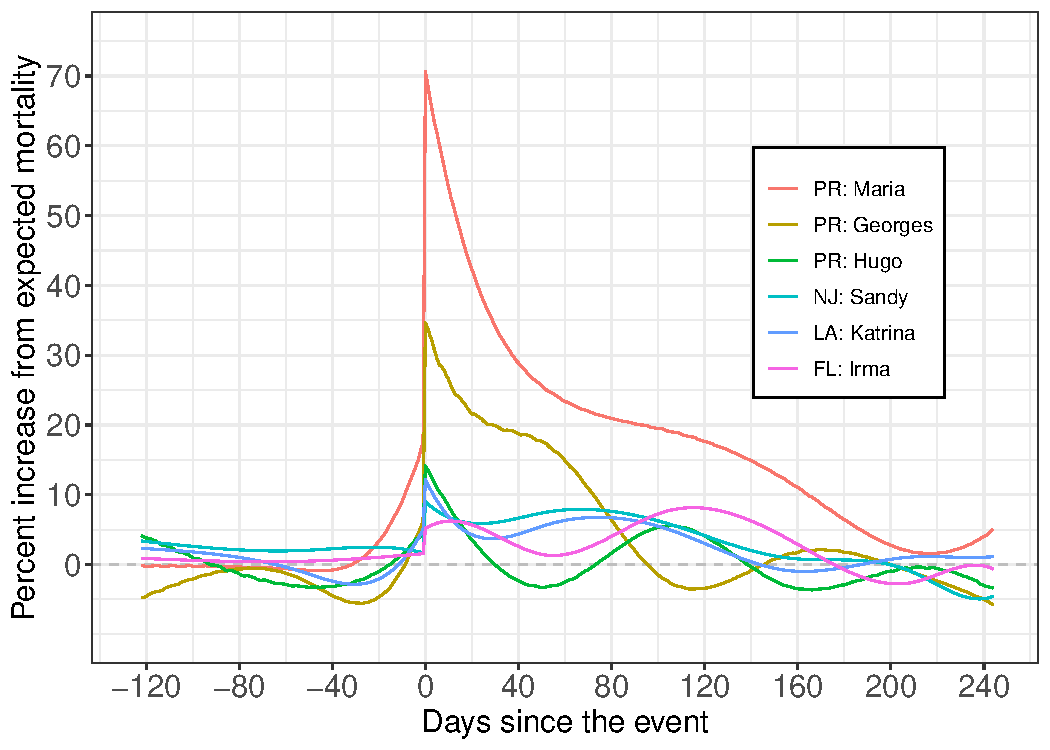
\includegraphics[width=1\linewidth]{figs/figure-1a.pdf} 
	\end{subfigure}&
	\begin{subfigure}[t]{0.30\linewidth}
		\centering
		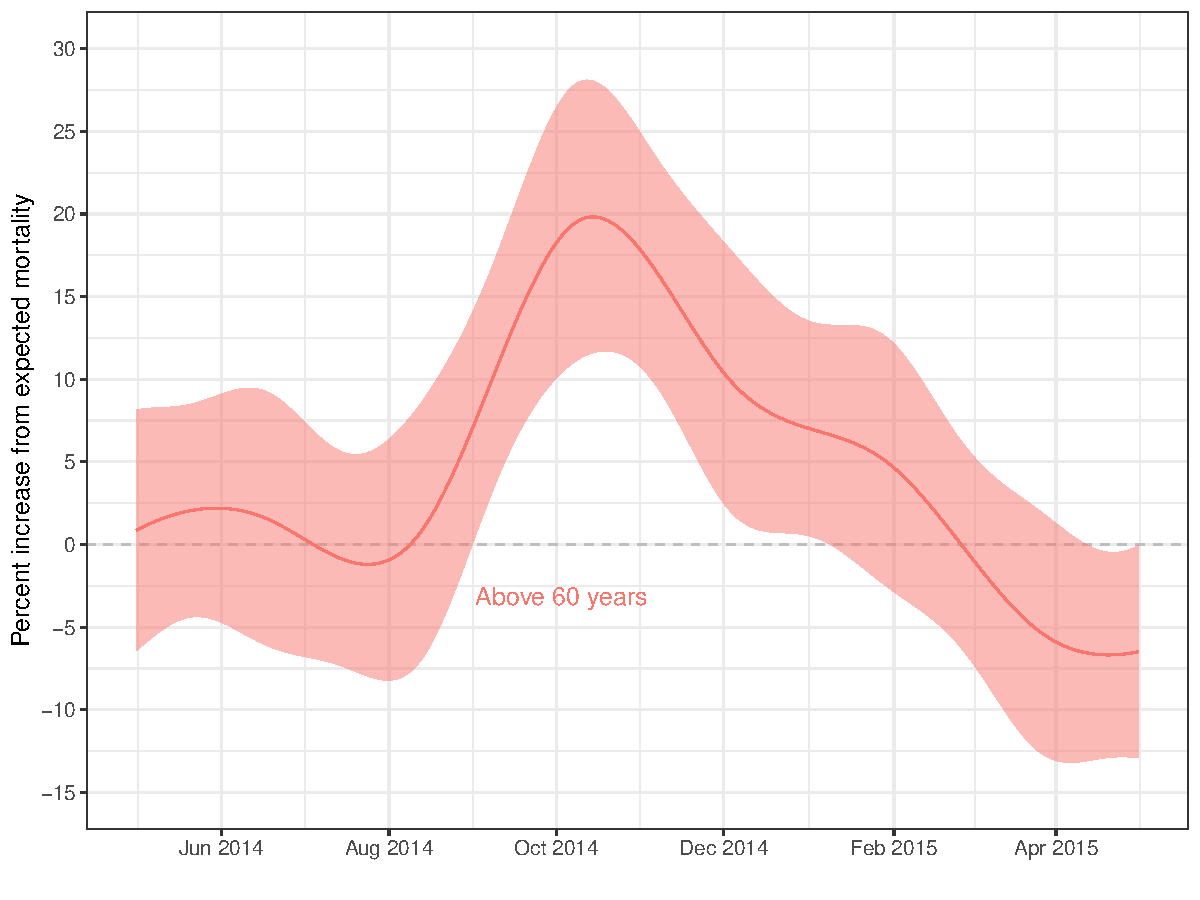
\includegraphics[width=1\linewidth]{figs/figure-1b.pdf}
	\end{subfigure}&
	\begin{subfigure}[t]{0.30\linewidth}
		\centering
		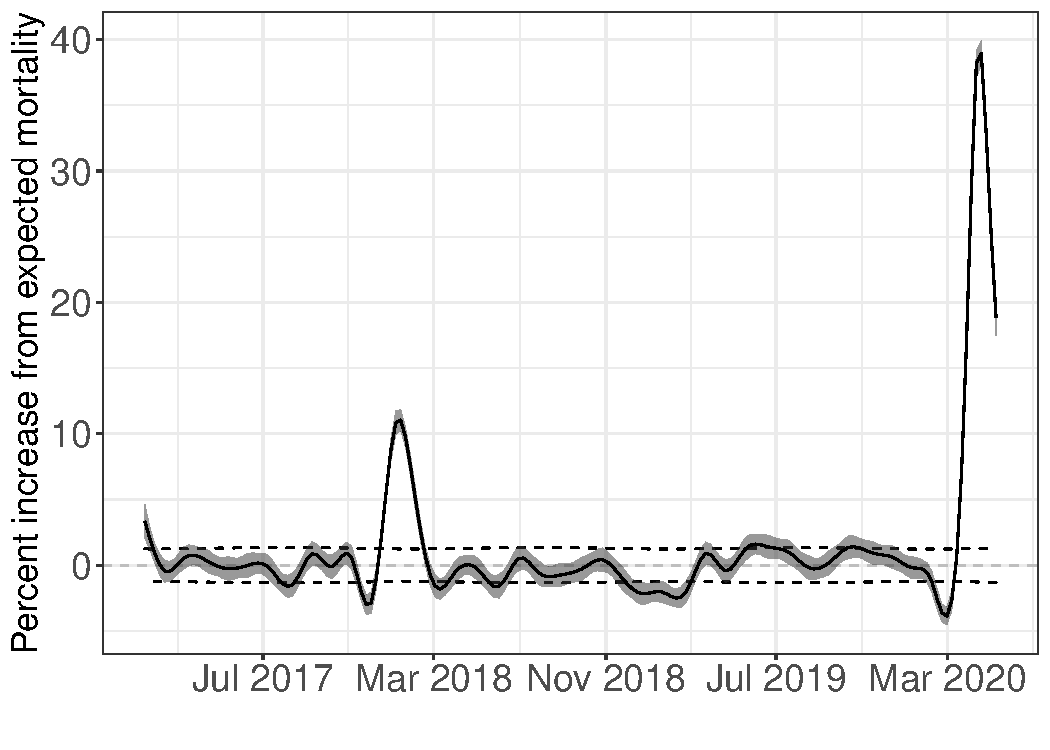
\includegraphics[width=1\linewidth]{figs/figure-1c.pdf}
	\end{subfigure}\\
    \end{tabular}
    \caption{Estimated event effects as percent increase over expected mortality. A) Comparison of six hurricanes. B) Estimated increase and point-wise confidence intervals among individuals 60 or over during the Chikungunya epidemic in Puerto Rico. C) Estimated increase and confidence interval for the the United States from January 2017 through May 2020.}
    \label{fig:fhat-estimates}
\end{figure}

\subsection{Quantifying the effects of epidemics}
\label{subsec:epidemics}
Our model can also be fitted to quantify the effects of epidemics or outbreaks. As an example, we fit our model to Puerto Rico mortality data from 2014-2015, when the Chikungunya outbreak occurred \cite{sharp2016surveillance, hsu2019risk}. We detected an increase in mortality rate for a period of 130 days for individuals over 60 years (Figure \ref{fig:fhat-estimates}B) and 160 days for the 0 to 4 years age group. We saw no noticeable effects for other age groups (Supplemental Figure \ref{supp-fig:chikungunya-agegroups}).

Although mortality data for the time period of the COVID-19 pandemic are not yet complete, the Center for Disease Control and Prevention (CDC) has implement a correction to the most recent counts and are making weekly state-level data from January 2017 to May 5, 2020 publicly available \cite{cdc2020covid19}. We fit our model to these data for each state and our event effect estimates clearly detects the COVID-19 pandemic for several states, as well as the 2018 flu epidemics (Figure \ref{fig:fhat-estimates}C, Supplemental Figure \ref{supp-fig:covid19-states}, \textbf{Table XXXX}). By aggregating the results for the entire United States we confirm that the COVID-19 pandemic had a substantially larger impact than the 2018 flu season. We also note that the difference is mostly driven by New York, New Jersey, Massachusetts, Michigan, and Illinois (Figure \ref{fig:excess-deaths}C, Supplemental Figure \ref{supp-fig:covid19-states}).

\subsection{Excess mortality estimates}
\label{subsec:excess-mortality}
Once we have fit our model, we can compute excess mortality estimates for any time period as well as standard errors that take into account, not just sample variability associated with count processes, but natural variation as well. We used the estimated parameters from the Puerto Rico data to compute excess deaths for the 365 days following the day hurricanes Georges, and Mar\'ia made landfall. We also computed these quantities for the 365 days following August, 2014, the first month that year for which we observe an increase for which a 99\% confidence interval do not include 0. Finally, we computed excess deaths in Puerto Rico during the COVID-19 pandemic, specifically from March 1, 2020 to April 7 2020. For María the excess death curve grew for XXX days with a point estimate on XXX of 3,264 (95\% CI: 2,820 to 3,709) XXX CORRECT???XX. For Georges the excess death curve grew for XX days witha point estimate of 1,293 (95\% CI: 1,013 to 1,572) XXFIX XX on XXX. We found excess deaths of 132 (95\% CI: 48 to 216), 1,293 (95\% CI: 1,013 to 1,572), and 3,264 (95\% CI: 2,820 to 3,709), respectively (Figure \ref{fig:excess-deaths}A). For the Chikungunya outbreak the excess death curve grows for XX days and then decreases until day XXX. The decrease is consistent with \emph{harvesting effect} [CITE https://academic.oup.com/aje/article/163/2/181/95820]. On XXX, when the excess death stabilizes, the point estimate was XXX [CI ]

Using the CDC data we computd excess mortality for the period of the COVID-19 pandemic for which we have data, specifically the March 8, 2020 to May 2, 2020 time period. When we compared these numbers to the reported numbers of COVID-19 deaths, we find a difference of 24,785 (95\% CI: 22,892 to 26,678) deaths (Figure \ref{fig:excess-deaths}B, \textbf{Table XX}). We also note that in the US, the number of excess deaths during the COVID-19 pandemic are much larger than the 2018 flu season, although this is not true for all states (Figure \ref{fig:excess-deaths}C, \textbf{Table XX}). Comparing to data from the New York Times \cite{smith2020coronavirus} we also note the reported COVID-19 deaths are under-counted in many states (\textbf{Table XX}).

\begin{figure}[ht]
	\begin{tabular}{lll}
	A&B&C\\
	\begin{subfigure}[t]{0.3\linewidth}
		\centering
		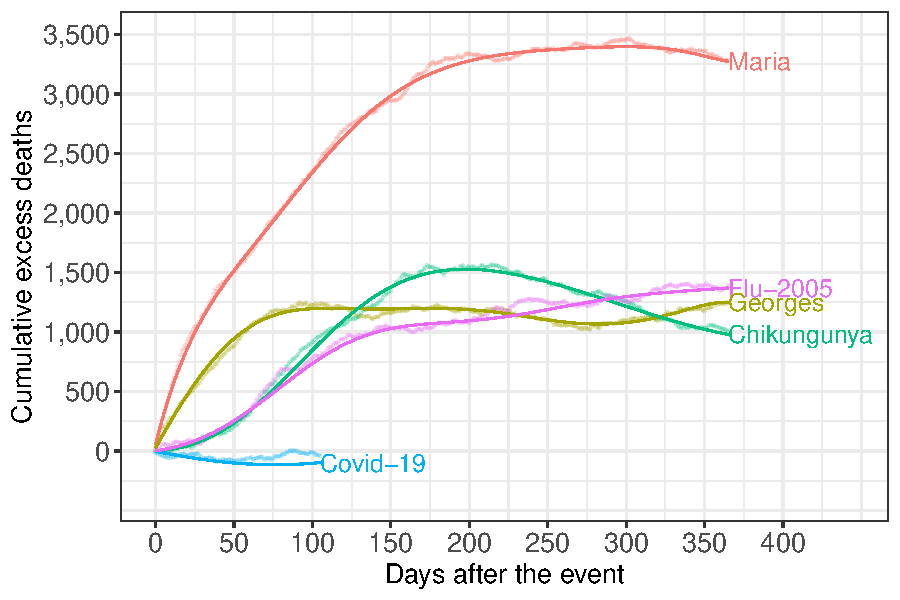
\includegraphics[width=1\linewidth]{figs/figure-2a.pdf} 
	\end{subfigure}&
	\begin{subfigure}[t]{0.3\linewidth}
		\centering
		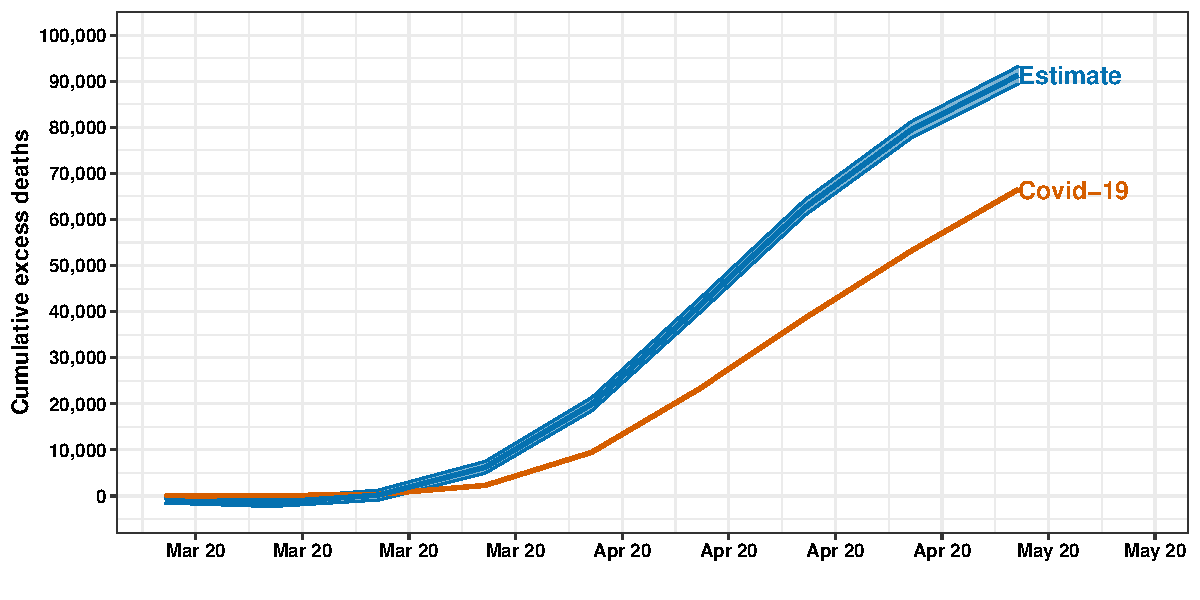
\includegraphics[width=1\linewidth]{figs/figure-2b.pdf}
	\end{subfigure}&
	\begin{subfigure}[t]{0.3\linewidth}
		\centering
		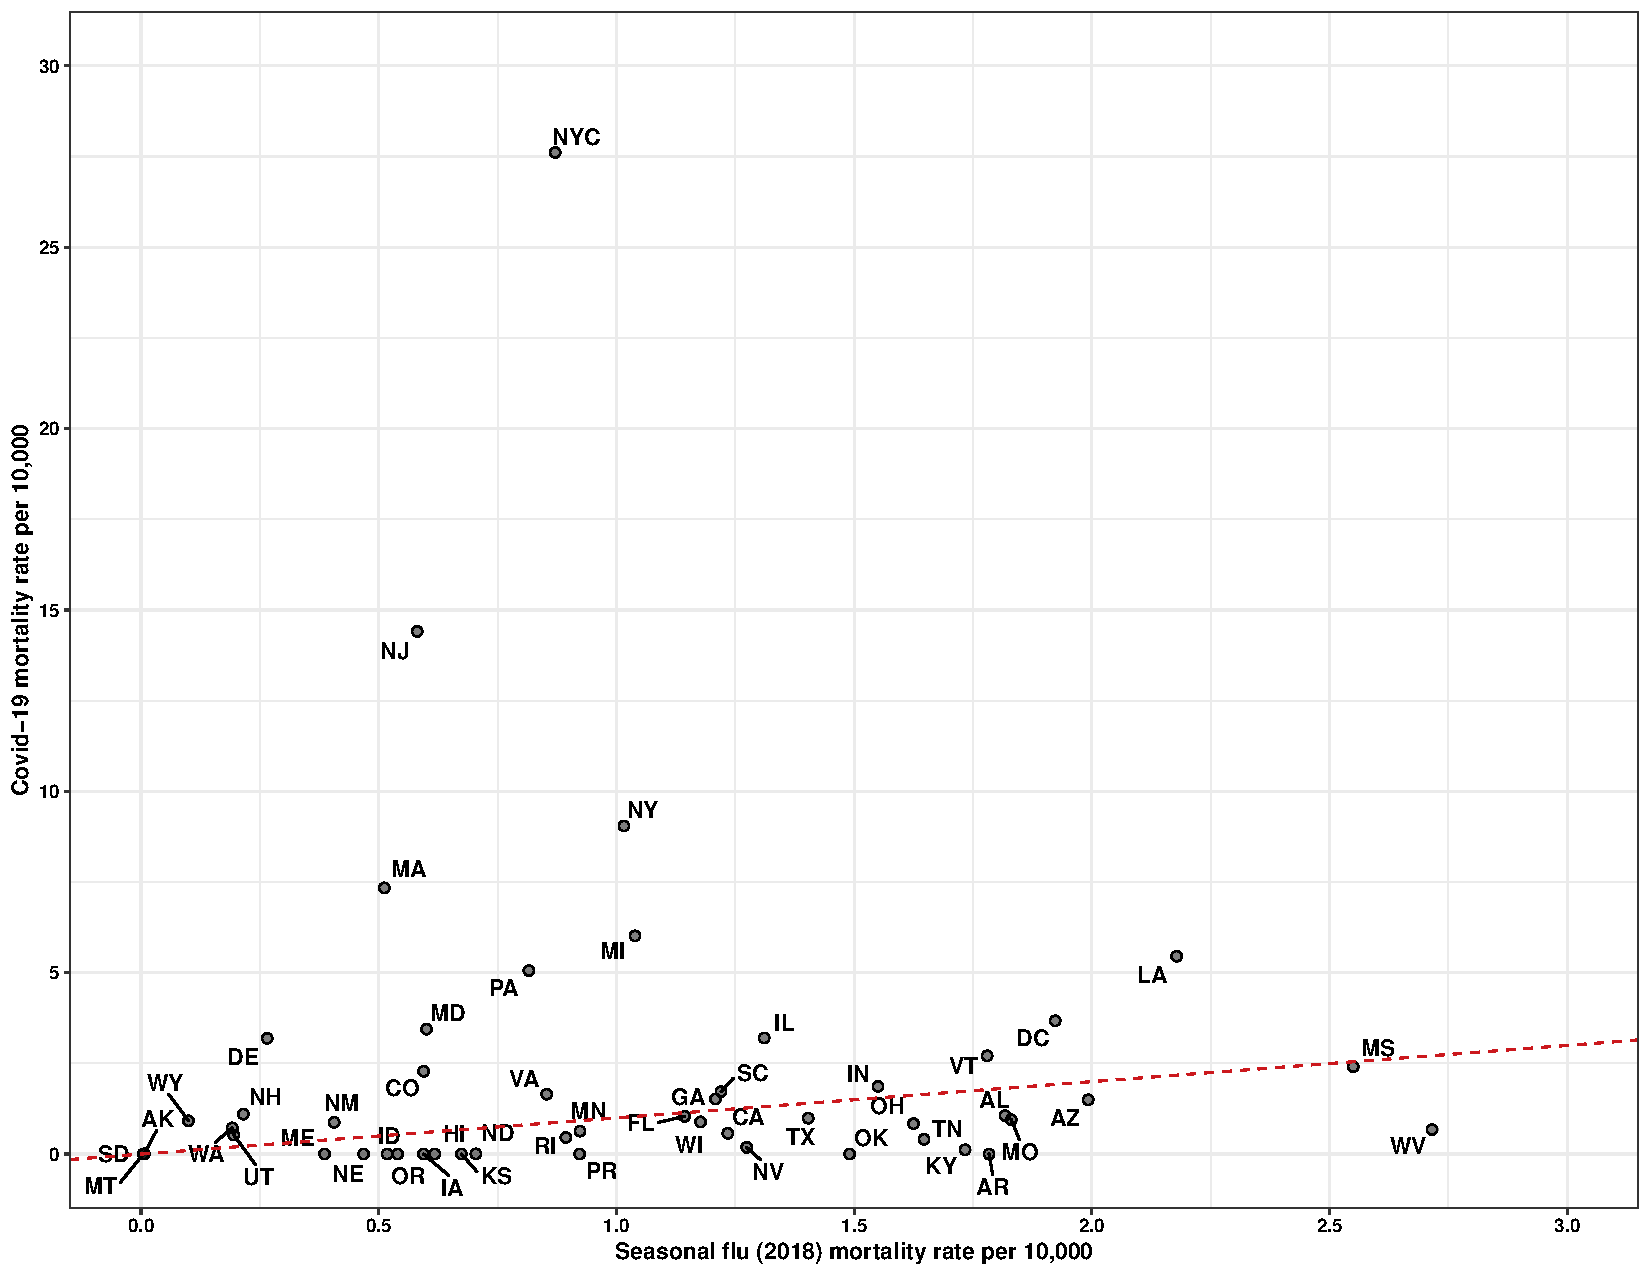
\includegraphics[width=1\linewidth]{figs/figure-2c.pdf}
	\end{subfigure}\\
	\end{tabular}
    \caption{Cumulative excess mortality estimates. A) Daily excess death estimates and 95\% confidence intervals for events in Puerto Rico starting on XXX, XX, XX, and XX for Hurricanes Georges, Hurricane María, the Chikungunya epidemic, and the COVID-19 pandemic, respectively.  B) Estimated cumulative excess mortality and reported COVID-19 cumulative deaths in the United States. C) State-specific cumulative excess mortality rates (excess deaths per 1,000 per 365 days) for COVID-19 plotted against the excess mortality rate 2018 Flu season. The identity line is represented in red and separates states in which mortality was higher during COVID-19 rom those in which the increase in mortality rate was where higher during the 2018 was worse. D) Cumulative excess mortality comparison between whites and blacks in Cook county, IL, with corresponding 95\% confidence intervals.}
    \label{fig:excess-deaths}
\end{figure}

\subsection{Across group comparisons}
\label{subsec:group-comparison}

The Cook County, IL, Medical Examiner's Office is making up-to-date records available online. This office investigates any human death in Cook County that falls within categories such as criminal violence, suicide, accident, diseases constituting a threat to public health, among unusual circumstances \cite{cookcovid19}. If we consider $\mu_t$ to be the expected number of deaths recorded by the Medical Examiner's Office, we can fit our model and interpret $f(t)$ as the percent increase in deaths examined by this office. We fit the model to these data and clearly observed the effects of the COVID-19 epidemic, in particular among individuals over 75. However, a persistent increase in mortality above normal levels is observed for individuals above 40. Since our model provides both estimates and standard errors of event effects, we can compare the effects for two or more groups and assess the statistical significance of the observed differences. Furthermore, we found a difference in the effect of the pandemic between white and black individuals in the months of March and April (Figure \ref{fig:cook-white-v-black}). 

Among those between 40 and 59 years of age, the percent increase in medical examiner death rates for Cook county was as high as 169\% (95\% CI: 134\% to 203\%) and 85\%  (95\% CI: 54\% to 115\%) on April 14 for whites and blacks, respectively, a statistically significant difference. Further, for the 60 to 74 age group we observed a peak percent increase of 630\% (95\% CI: 544\% to 716\%) and 497\% (95\% CI: 424\% to 571\%), respectively. Finally, the percent increase for individuals 75 years and older was 2,334\% (95\% CI: 2,056\% to 2,612\%) and 1213\% (95\% CI: 1092\% to 1334\%), respectively, another statistically significant finding (Figure \ref{fig:cook-white-v-black}).  The population size for other racial groups was substantially smaller and were not included in the analysis.

\begin{figure}[ht]
	\centering	
		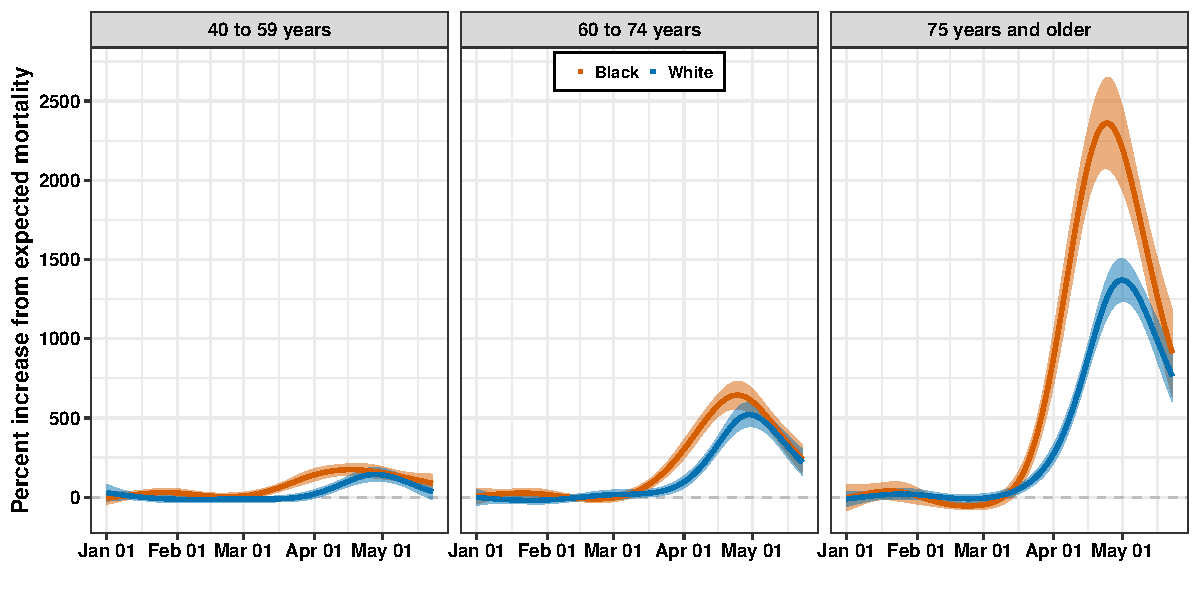
\includegraphics[width=1\linewidth]{figs/figure-3.pdf} 
	\caption{Comparison of estimated percent increase in mortality in Cook county, IL, for individuals above 40 between whites and blacks with corresponding 95\% confidence intervals.}
	\label{fig:cook-white-v-black}
\end{figure}

% Although only about \textbf{1/5XXX} of all deaths are examined by the medical examiner, one of the criteria for an examination from this office is that the cause of death is a disease constituting a threat to public health, which implies that some if not most COVID-19 deaths are being examined. This database includes demographic information permitting comparisons among, for example, racial groups. The largest percent increases were observed for individuals over 65 \textbf{(Supp Fig X)}. Among those 65 years of age and older, the increase in medical examiner death rate for Cook county was as high as \textbf{XXX} on \textbf{XXXX} and shows a significant difference between black and white populations. The population size for other racial groups of this age was substantially smaller and were not included in the analysis.
 
% disease reached Puerto Rico and our excess death method reveals that in the month of XX there were XXX deaths among people over 60, v is an arbovirus common to tropical regions, mainly in Africa and Asia. According to XXX, most infected individuals recover 10 days, and deaths are rare. In 2014 the disease reached Puerto Rico and our excess death method reveals that in the month of XX there were XXX deaths among people over 60, very likely due to a Chikungunya outbreak. The next XX months saw an incread in the death rate of individuals over 60  (Supplemental Figure 1b) as well as in infants (Supplemental Figure 1b)  with a final excess mortality count of XXXX  +/- XXXX (Supplemental FIgure 1c).

\subsection{Relative proportion of specific causes of death can be used with incomplete data}
\label{subsec:causes-deaths}
Limitations of our approaches for detecting and monitoring health crises are that it requires 1) complete death count data and 2) an estimate of population displacement. Note that incomplete death counts or underestimates of population displacement will result in underestimate of the death rate. However, if we redefine $Y_t$ as the number of deaths do to a specific cause at time $t$ and $N_t$ as the total number of recorded deaths at time $t$, then the estimate of $f$ can be interpreted as the percent increase in the proportion of deaths due to that cause, even if the data is incomplete. The underlying cause of death for the Puerto Rico mortality data was coded using the International Classifications of Diseases tenth revision (ICD 10) \cite{world2004icd}. We denote all ICD 10 codes between A00 and A79 as bacterial infections and using the approach described above we find that deaths attributable to this cause were elevated for at least 2 months after the landfall of hurricane Mar\'ia in Puerto Rico (Figure \ref{fig:fhat-bacteria}). A similar index for respiratory diseases computed for the COVID-19 pandemic shows no anomalies (Supplemental Figure \ref{supp-fig:respiratory-index-pr}).

\begin{figure}[ht]
	\centering	
		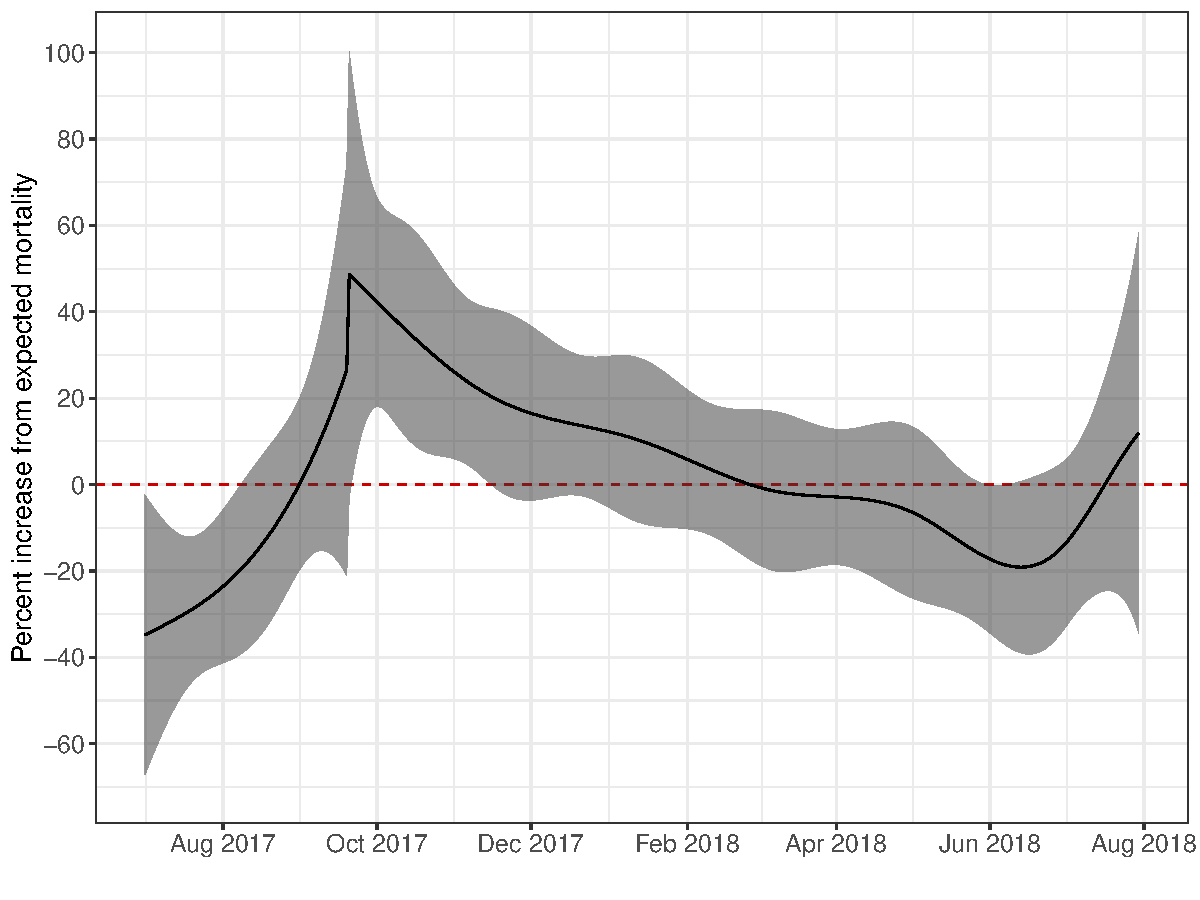
\includegraphics[width=1\linewidth]{figs/figure-4.pdf} 
	\caption{Bacterial infections mortality index. The solid-black line corresponds to the percent change in proportion of mortality, $\hat{f}(t)$, caused by bacterial infections. The shaded area represents a 95\% confidence interval for $\hat{f}(t)$. Bacterial infections were defined as all ICD 10 codes between A00 and A79.}
	\label{fig:fhat-bacteria}
\end{figure}

\subsection{Natural Variability and Correlated Counts}
\label{subsec:natural-variability}
\begin{itemize}
% Need to finish this section
    \item Do previous methods take this into account? If not write a paragraph showing it is necessary
    \item The variance is 0.05
    \item Plot of ACF
\end{itemize}

\section{Methods}
\label{sec:methods}

\subsection{Mortality Data}
\label{subsec:mortality-data}
We obtained detailed mortality and population size data related to hurricanes Hugo, Georges, and Maria in Puerto Rico, Katrina in Louisiana, Sandy in New Jersey, and Irma in Florida. For Puerto Rico, we requested individual level mortality information with no personal identifiers from the Department of Health of Puerto Rico and obtained individual records including date, gender, age, municipality, and cause of death from January 1985 to May 2020. We used this data to construct daily death counts for different strata of the Puerto Rican population throughout the study period. We also requested daily death counts from Florida, New Jersey, and Louisiana’s Vital Statistic systems and obtained data from January 2015 to December 2018, January 2007 to December 2015, and January 2003 to December 2006, respectively. Note that we did not ask for individual records from these jurisdictions.

We also obtained estimates of excess deaths made public on May 12, 2020 by the CDC \cite{cdc2020covid19}. This dataset included weekly estimates of death counts for each state and Puerto Rico for the period of January 2017 and May 2020. Furthermore, we obtained individual level mortality data from the Cook County, IL, medical examiner office \cite{cookcovid19}. These data included demographic information for each death including age, sex, and race.

\subsection{Population Estimates}
\label{subsec:population}
Yearly population estimates for Puerto Rico were obtained from the Puerto Rico Statistical Institute. Yearly population estimates for other US states were obtained from the US Census bureau. We computed daily population estimates via linear interpolation of the available data. To obtain an estimate of the population displacement after Hurricane Maria in Puerto Rico, we use population proportion estimates from Teralytics (Supplemental Figure \ref{supp-fig:pop-displacement-pr}).

\subsection{Statistical model}
\label{subsec:statistical-model}
We assume the mortality counts at $t$ follows a generalized linear mixed model defined above in the Results section. Specifically, we assume:
\begin{equation*}
    Y_t \mid \varepsilon_t \propto \mbox{Poisson}[ \mu_t \{1 + f(t)\}  \varepsilon_t ], \mbox{ for } t = 1, \dots,T 
\end{equation*}
where the expected counts have the form:
\begin{equation*}
    \mu_t =N_t  \exp[\alpha(t) + s(t) + w(t)]
\end{equation*}
and the vector $[\varepsilon_1, \ldots, \varepsilon_T]^\top$ has a multivariate normal distribution with mean 1 and variance-covariance matrix $\Sigma$ determined by an auto-regressive (AR) process of order $p$:
\begin{equation*}
    \Sigma = \sigma^2
    \begin{pmatrix} 1 & \rho_1 & \rho_{2} & \dots & \rho_{T} \\ 
    \rho_{1} & 1 & \rho_{1} & \ldots & \rho_{T-1} \\
    \vdots & \vdots & \vdots & \vdots & \vdots \\
    \rho_{T} & \rho_{T-1} & \rho_{T-2} & \dots & 1 \\ 
    \end{pmatrix}
\end{equation*}
Here $\sigma$ corresponds to the year-to-year standard deviation and $\rho_h$ is the auto-correlation of two error terms that are $h$ time units from each other. In practice, obtaining Maximum Likelihood Estimates (MLE) for this model is not straight-forward, in particular because the flexibility in $f(t)$ and $\Sigma$ makes the model non-identifiable in practice. We now describe a three step approach that works well in practice, as demonstrated both by simulation and empirical validation.

We start by modeling the yearly trend $\alpha(t)$ with natural cubic splines with a knot every five years. We model the seasonal effect $s(t)$ with a harmonic model with at most 3 harmonics. Finally
\begin{equation*}
    w(t) = [w_1, \ldots, w_7] \times \boldsymbol{1}_{t \bmod 7==k} \mbox{ where } \sum_{k=1}^7 w_k = 0
\end{equation*}
represents seven constrained parameters, one for each day of the week. Because natural disasters and outbreaks are rare, we assume that $f(t)$ is 0 for the majority of our dataset. This implies that for the majority of time points
\begin{equation*}
    Y_t \mid \varepsilon_t \propto \mbox{Poisson}(\mu_t  \varepsilon_t )
\end{equation*}
This implies that, for example, for $N = T / 365$ years of daily data we would have $T$ data points to fit a model with at most N/5 + 6 + 6 + 1 parameters for the mean model. For five years of data this translates into 1,825 data points and 14 parameters. This implies that we can obtain highly precise estimates even in the presence of the extra dispersion introduced by $\varepsilon$. We therefore fit a Poisson Generalized Linear Model to regions that we know do not include natural disasters or outbreaks and consider the MLE $\hat{\alpha}(t)$, $\hat{w}(t)$, and $\hat{s}(t)$ as fixed.

In the second step we estimate $\Sigma$, and to do this we select a control region that is continuous for which we know $f(t)=0$. To estimate the $\sigma^2$ and the autoregressive parameters we can use the law of total variance to note that the observed percent change from the mean
\begin{equation*}
    r_t = \frac{Y_t - \mu_t}{\mu_t}
\end{equation*}
has expected value and variance
\begin{equation*}
    \mathbb{E}\left(r_t \right) = 0 \mbox{ and } \mbox{Var}\left(r_t\right)= \sigma^2 + 1/\mu_t
\end{equation*}
Intuitively, these two components are the variance added by $\varepsilon$ and the Poisson variability respectively. The above implies that if we define the transformation:
\begin{equation*}
    Z_t = \frac{r_t}{\sqrt{\mbox{Var}\left(r_t\right)}}
\end{equation*}
we have an approximately normally distributed random variable with the same correlation structure as $\varepsilon_t$, which is what we want to estimate. We use the Yule-Walker equation approach to estimate AR process parameters. To estimate $\sigma^2$ we use:
\begin{equation*}
    \hat{\sigma}^2 = \max\left\{ \frac{1}{T}\sum_{t=1}^T  \left(\frac{Y_t - \hat{\mu}_t}{\hat{\mu}_t}\right)^2  - \frac{1}{\mu_t}, \, 0\right\}
\end{equation*}
Using these estimates we can form an estimate $\hat{\Sigma}$ which we will consider known in the next step.

In the third step we treat this covariance as known, assume $f(t)$ can be modeled as a natural cubic spline, and use iteratively re-weighted least squares to obtain an estimate $\hat{f}(t)$. To account for non-continuities due to direct effects from natural disasters we permit the spline to be discontinuous at the event day. 

\subsection{Approximation for uncorrelated data}
Note that our model can be easily adapted to be fitted to weekly data. In this case there is no need to include weekday effect parameters nor a correlation structure for the errors. We find that fitting an overdispersed generalized linear model provides practically equivalent results as the more complex GLMM and therefore we use it for weekly data, as well as other datasets in which there does not appear to be correlated counts.

\subsection{Excess death estimates}
\label{subsec:excess-deaths}
To estimate excess deaths we must first determine a period of interest, here we propose two approaches. First one can take the conventional approach and determine a period of interest based on subject matter knowledge (e.g., months constituting the flu season for a particular year). Otherwise one can use what we refer to as the \textit{period of indirect effect}. Define the interval starting on the event day (e.g., landfall for a hurricane), denoted here with $t_0$, until the first day, $t > t_0$, for which $f(t)=0$. Since $f(t)$ is unobserved, and instead we obtain an estimate we take the conservative approach of defining the end of the period when the lower bound of a 95\% confidence interval reaches 0 $\left(\mbox{i.e., } \hat{f}(t)-1.96\hat{\mbox{se}}\{\hat{f}(t)\}=0\right)$. We denote the period of interest with $I$ and define \textit{fitted} and \textit{observed} excess deaths at time $t$ with $\hat{\mu}_t \hat{f}(t)$ and $Y_t - \hat{\mu}_t$, respectively. Finally, cumulative excess deaths are estimated by adding the excess deaths of each day in $I$: 
\begin{equation*}
    \mbox{Excess deaths} = \sum_{t \in I} \hat{\mu}_t \hat{f}(t) 
\end{equation*}
We construct a 95\% confidence interval with:
 \begin{equation*}
    \mbox{Var(Excess deaths)} = \sum_{t_ \in I} \hat{\mu}_t^2 \mbox{ Var}\left(\hat{f}(t)\right)
 \end{equation*}
 
\subsection{Counterfactual considerations}
Estimation of excess mortality requires an accurate prediction of the counterfactual scenario of no event. As stated above, for periods of no events our approach simplifies to:
\begin{equation*}
    Y_t \mid \varepsilon_t \propto \mbox{Poisson}(\mu_t  \varepsilon_t )
\end{equation*}
This implies that, for example, the counterfactual of no hurricane in Puerto Rico for hurricane Mar\'ia is determined by model \ref{eq:mean-model}. It is well known that population displacement may occur after natural disasters \cite{mbaye2017climate, thomaz2013post, curtis2015recovery}. Therefore, the mortality and population distributions differ between the factual and counterfactual scenarios. In the past, the inability to measure population displacement in close to real time has limited researchers to use the same population estimates in both factual and counterfactual scenarios. However, with the advent of social media data and call detail records, we now have the ability to estimate population displacement shortly after a disaster. Assuming population displacement in Puerto Rico after hurricane Mar\'ia (Supplemental Figure \ref{supp-fig:pop-displacement-pr}) in both the factual and counterfactual scenarios we find the elevated and persistent increase in mortality described in the Results section (Figures \ref{fig:fhat-estimates}A \& \ref{fig:excess-deaths}A). Not accounting for population displacement in both the factual and counterfactual scenarios yields a noticeable yet non significant difference in our estimates (Supplemental Figure \ref{supp-fig:counterfactual-considerations}). Assuming that the population displacement observed post-hurricane was caused by the disaster, one can postulate that the counterfactual scenario should not account for population displacement. 

\subsection{Simulation study}
To assess that our estimation procedure produces useful results we conducted a Monte Carlo simulation. Specifically, we computed $\hat{\mu}_t$ for $t=1,\ldots, T$, using the Puerto Rico mortality data with model (\ref{eq:mean-model}) and generated data $Y_t^* \sim \mbox{Poisson}(\hat{\mu}_t)$ with serial correlation. We considered three scenarios: 1) a hurricane-like event where we expect mortality to increase rapidly and stay above normal levels for some time, 2) an epidemic-like event in which mortality increases slowly until reaching some plateau and then decreasing to normal levels, and 3) a time period of no event in which we expected our estimate of $f(t)$ to be centered around 0. Parameters describing our simulation are in \textbf{Supplemental Table XX}. Our implementation produces accurate and precise results for both $f$ and $\Sigma$ (Supplemental Figure \ref{fig:simulation}).

% To confirm that our estimation procedure produces useful result we conducted a Monte Carlo simulation. Specifically, we generated data from the model above with parameters described in \textbf{Supp Tab XX} and \textbf{Supp Fig XX}. Our procedure produces accurate and precise results for both $f$ and $\Sigma$ \textbf{(Supp Figure)}

We also performed an empirical test by estimating excess deaths and the standard error for period for which no natural disaster occured and no known outbreak. In this case the the estimate divided by its standard error should follow a normal distribution.  We find that the model with correlated errors performs best with the Poisson model greatly underestimating the standard error. Adding a over-dispersion parameter improves the results but still underestimates the variance \textbf{(Supp Figure)}. Providing further evidence that considering correlation is important when analyzing daily data.

\section{Discussion}

\section{Conclusion}

% We first determined the period of indirect effect for each hurricane. To do this, we defined the interval starting on landfall day, denoted here with $t_0$, until the first day, $t_{ij} > t_0$, for which $f(t_{ij})>0$. Because we do not observe $f(t_{ij})$, and instead obtain an estimate we took the conservative approach of defining the period with the day for which the lower part of a marginal 95\% confidence interval crosses 0: $f(t_{ij})−1.96\hat(se)\{\hat{f}(t_{ij})\}>0$. We denoted this interval with $I$ and defined the excess deaths by adding the observed deaths minus expected deaths for every day in the interval:
% \begin{equation*}
%     \mbox{Excess deaths} = \sum_{t_{ij} \in I} \left[Y_{ij} − N_{ijk}\exp\{g_k(t_{ij})+s_k(j)\}\right]
% \end{equation*}
%  We construct a 95\% confidence interval using the following approximation for the Poisson model:
%  \begin{equation*}
%     \mbox{Var(Excess deaths)} = \sum_{t_{ij} \in I} N_{ijk}\exp\{g_k(t_{ij})+s_k(j)\}
%  \end{equation*}
 
\newpage
\bibliographystyle{unsrt}
\bibliography{ref.bib}

\newpage
\begin{center}
\LARGE{\textbf{Supplemental Material}}
\end{center}

% Supp figure 1: Trend and seasonal components
\begin{suppfigure}[ht]
	\begin{tabular}{lll}
	A&B\\
	\begin{subfigure}[t]{0.49\linewidth}
		\centering
		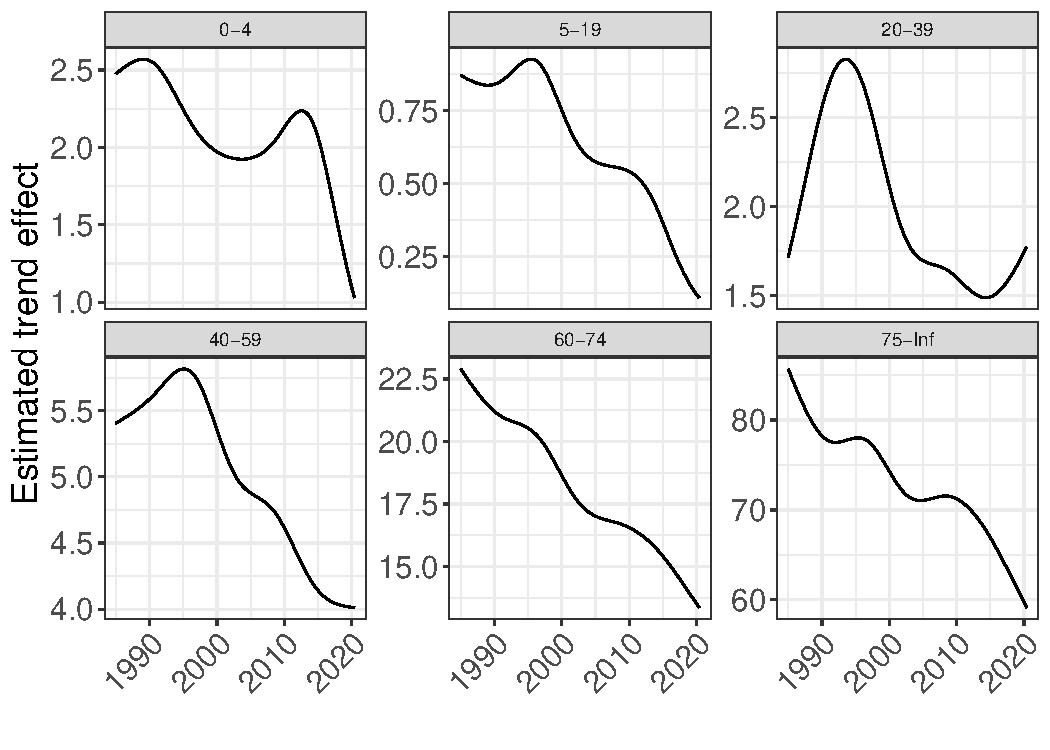
\includegraphics[width=1\linewidth]{figs/supp-figure-1a.pdf} 
	\end{subfigure}&
	\begin{subfigure}[t]{0.49\linewidth}
		\centering
		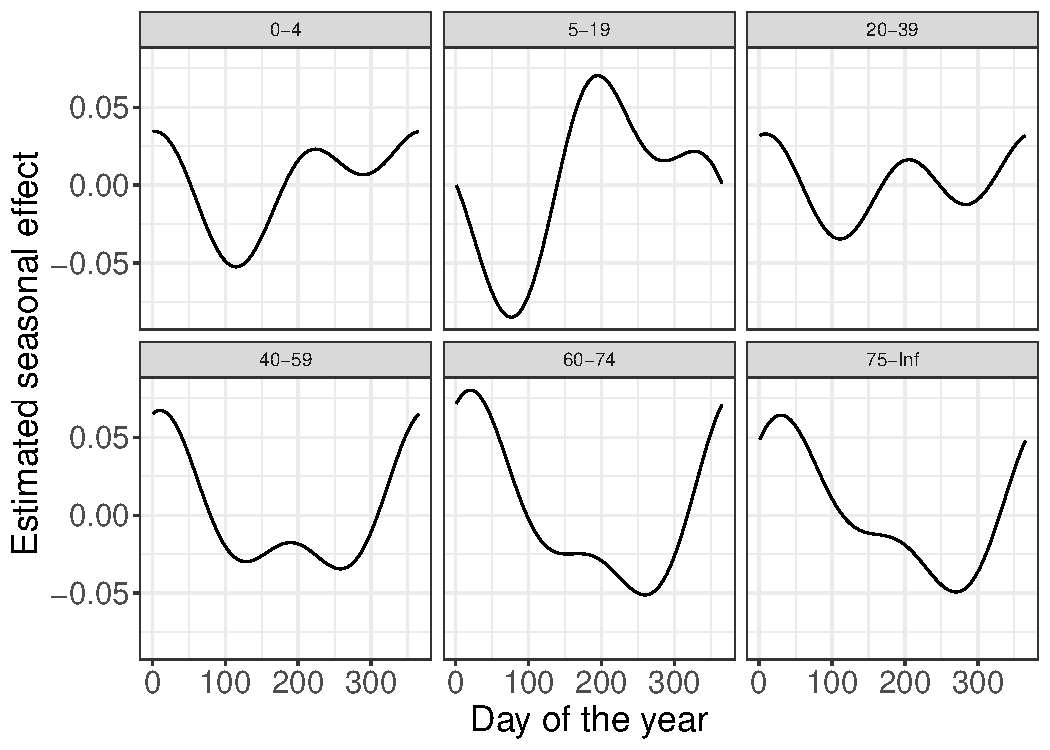
\includegraphics[width=1\linewidth]{figs/supp-figure-1b.pdf}
	\end{subfigure}&\\
    \end{tabular}
    \caption{Estimated trend and seasonal components of model \ref{eq:mean-model} for six age groups in Puerto Rico. A) Trend component for each age group in Puerto Rico. This corresponds to the yearly mortality rate per 1,000. B) Seasonal component for each age group.}
    \label{supp-fig:model-components}
\end{suppfigure}

% Supp figure 2: QQ plots and ACF
\begin{suppfigure}[ht]
	\begin{tabular}{lll}
	A&B\\
	\begin{subfigure}[t]{0.49\linewidth}
		\centering
		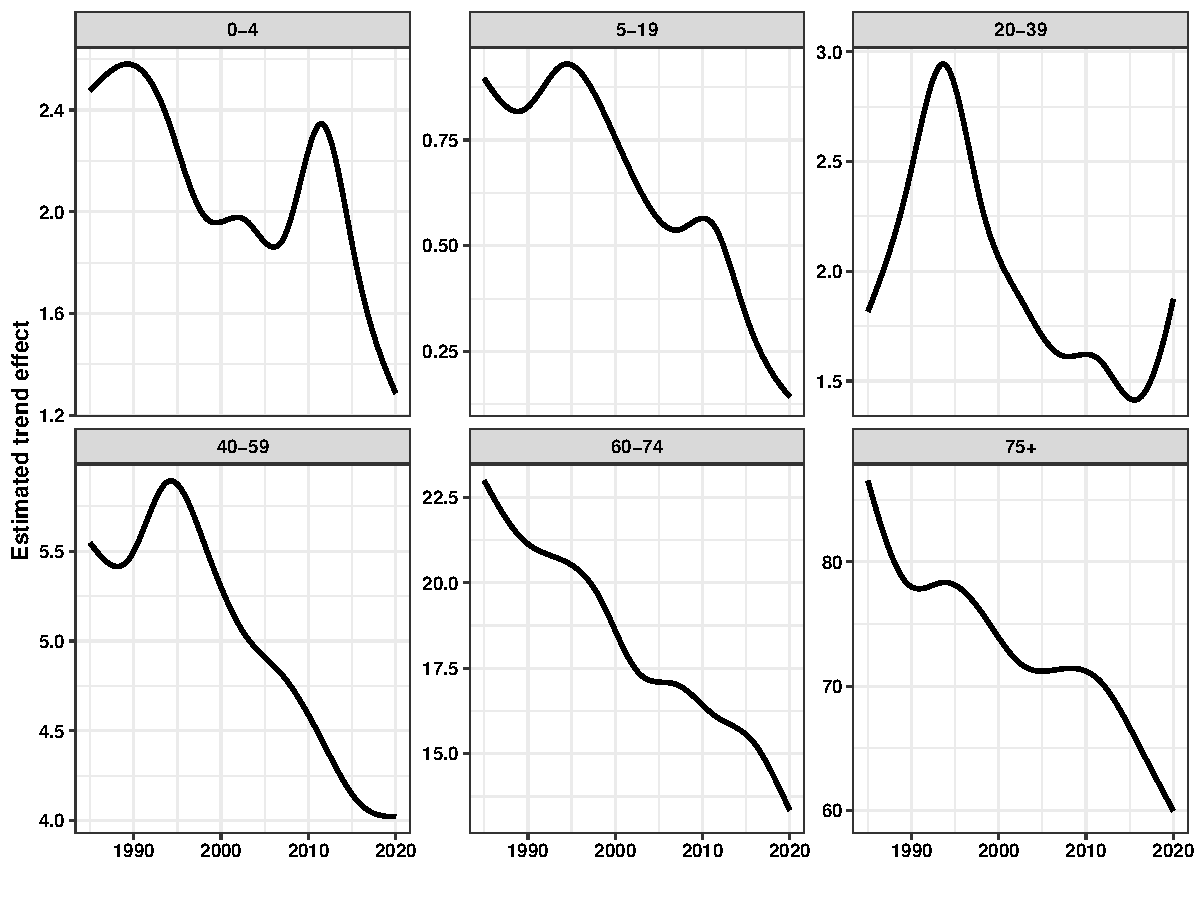
\includegraphics[width=1\linewidth]{figs/supp-figure-2a.pdf} 
	\end{subfigure}&
	\begin{subfigure}[t]{0.49\linewidth}
		\centering
		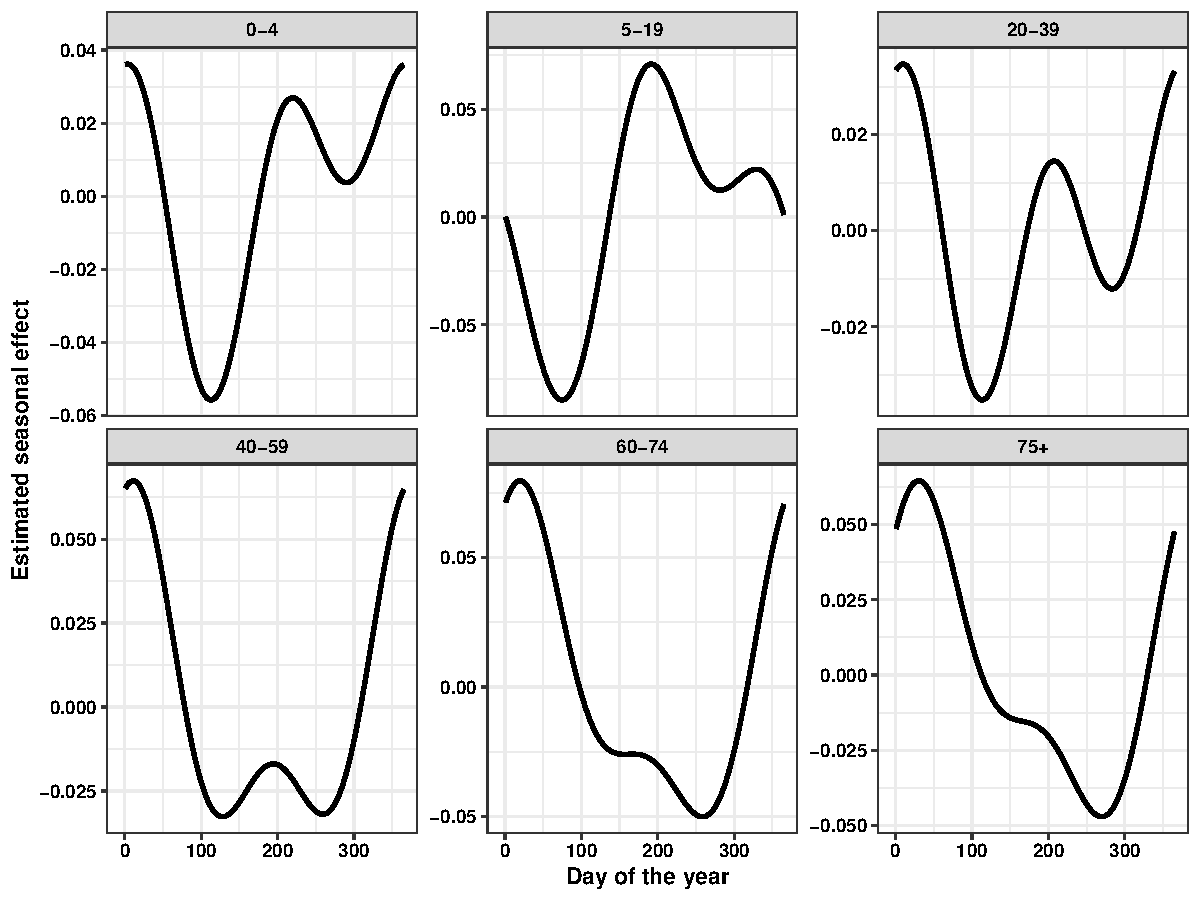
\includegraphics[width=1\linewidth]{figs/supp-figure-2b.pdf}
	\end{subfigure}&\\
	C&D\\
	\begin{subfigure}[t]{0.49\linewidth}
		\centering
		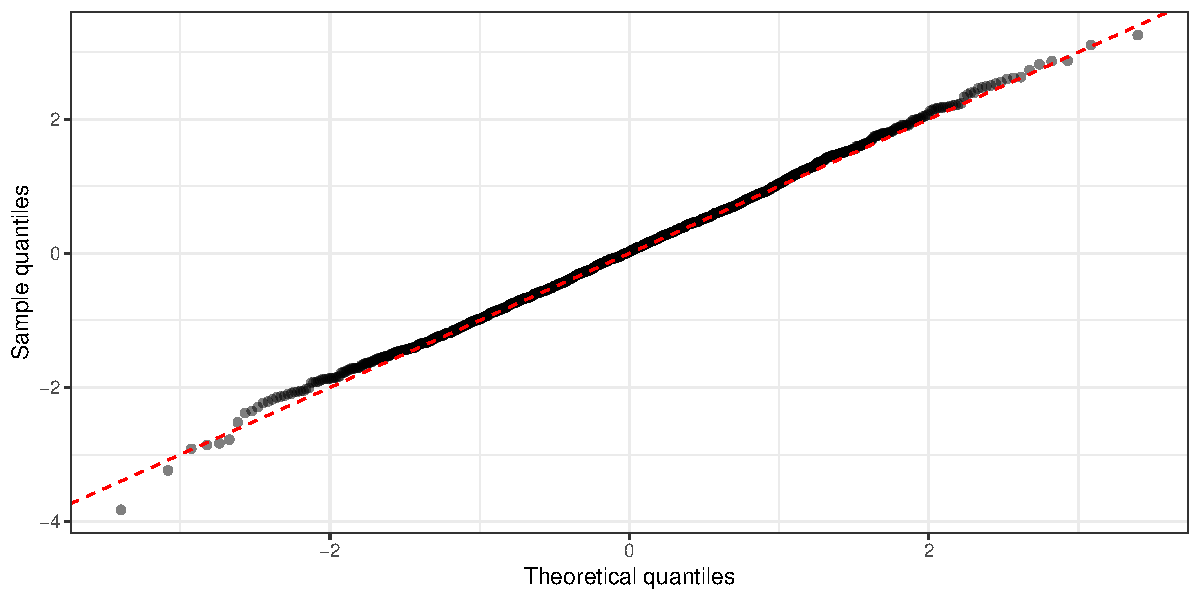
\includegraphics[width=1\linewidth]{figs/supp-figure-2c.pdf}
	\end{subfigure}&
	\begin{subfigure}[t]{0.49\linewidth}
    	\centering
	    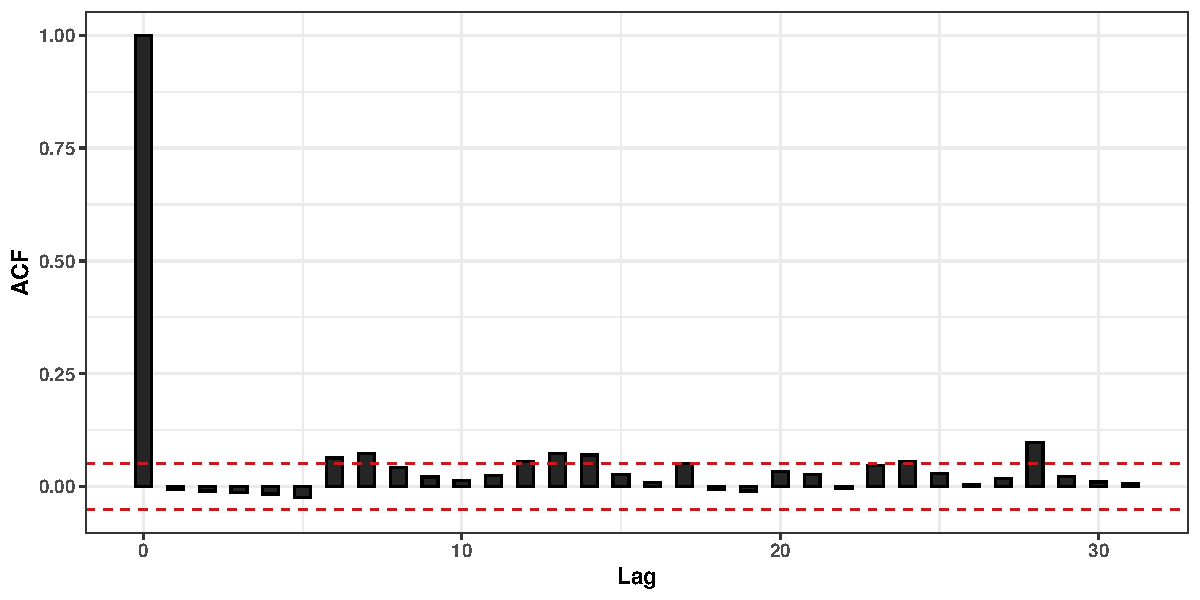
\includegraphics[width=1\linewidth]{figs/supp-figure-2d.pdf}
    \end{subfigure}\\
    \end{tabular}
    \caption{Model assessment. We defined a control period where $f(t)=0$ and assess distributional assumptions in the naive scenario when serial correlation is not adjusted for and when it is. A) Quantile-quantile plot of Pearson residuals without adjusting for serial correlation. B) Autocorrelation plot of observed data, the red-dash lines represent a 95\% confidence interval centered at zero. C) Quantile-quantile plot of Pearson residuals when adjusting for serial correlation. D) Autocorrelation plot of data adjusted for serial correlation, the red-dash lines represent a 95\% confidence interval centered at zero.}
    \label{fig:correlated-errors}
\end{suppfigure}

% Supp figure 3: F hat for all six hurricanes
\begin{suppfigure}[ht]
	\centering
	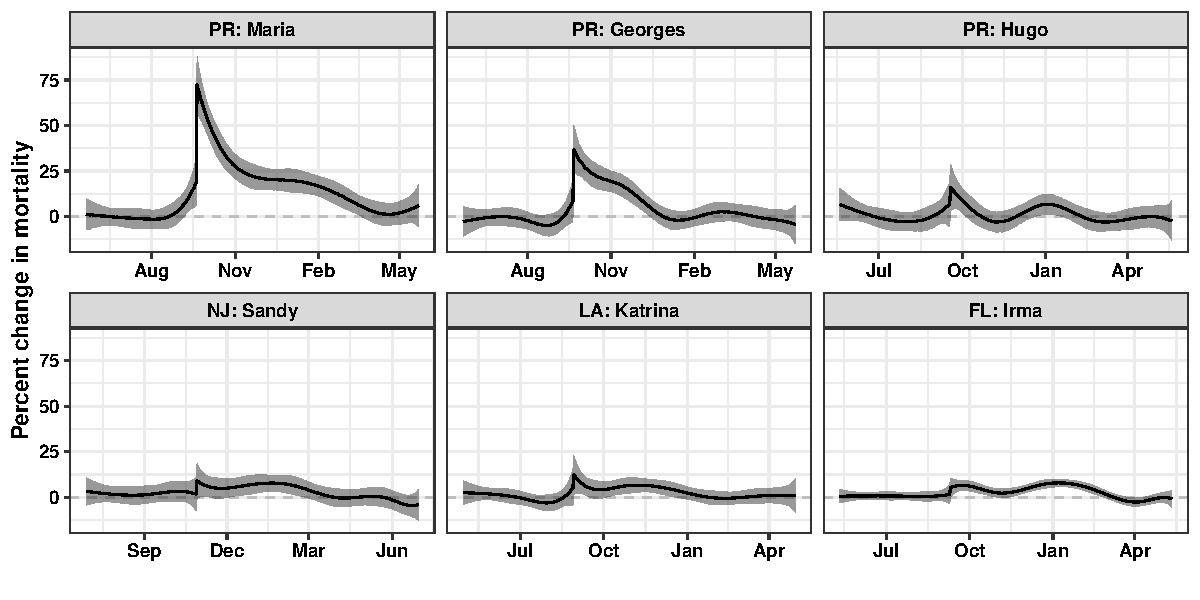
\includegraphics[width=1\linewidth]{figs/supp-figure-3.pdf} 
    \caption{Estimated event effects as percent increase over expected mortality for the six hurricanes.}
	\label{supp-fig:hurricane-effects}
\end{suppfigure}

% Supp figure 4: Fhat for age groups during chikungungya
\begin{suppfigure}[ht]
	\centering
	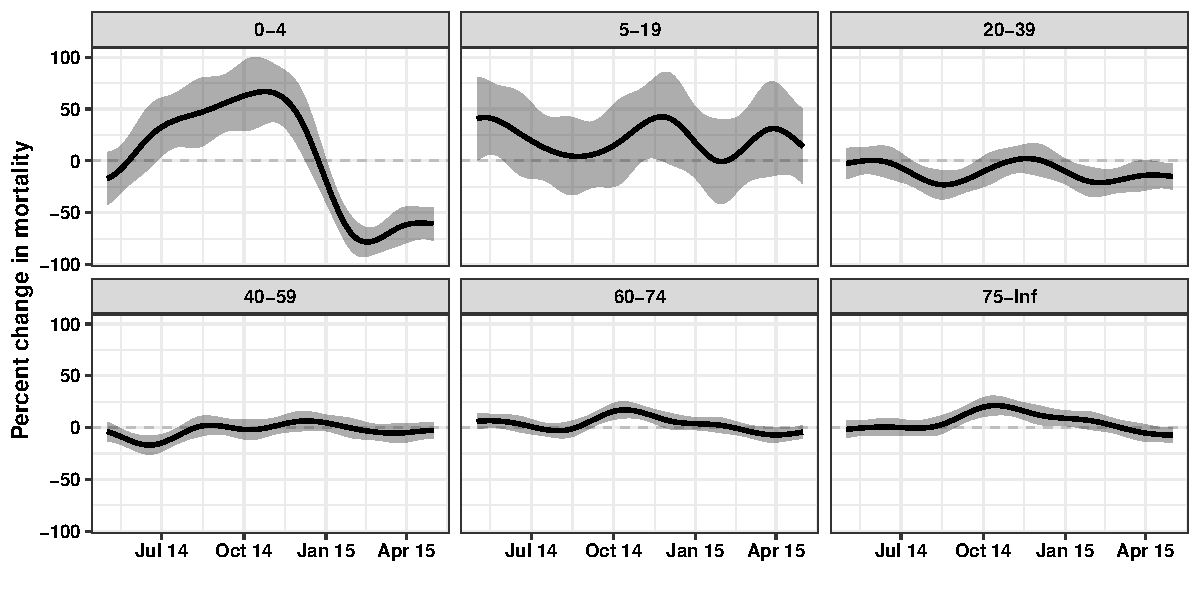
\includegraphics[width=1\linewidth]{figs/supp-figure-4.pdf} 
    \caption{Estimated event effects as percent increase over expected mortality during the Chikungunya epidemic in Puerto Rico for six age groups. The points are percetage above or below expectation for the daily counts.}
	\label{supp-fig:chikungunya-agegroups}
\end{suppfigure}

% Supp figure 5: Top 12 jurisdiction most affected by covid 19 in USA
\begin{suppfigure}[ht]
	\centering
	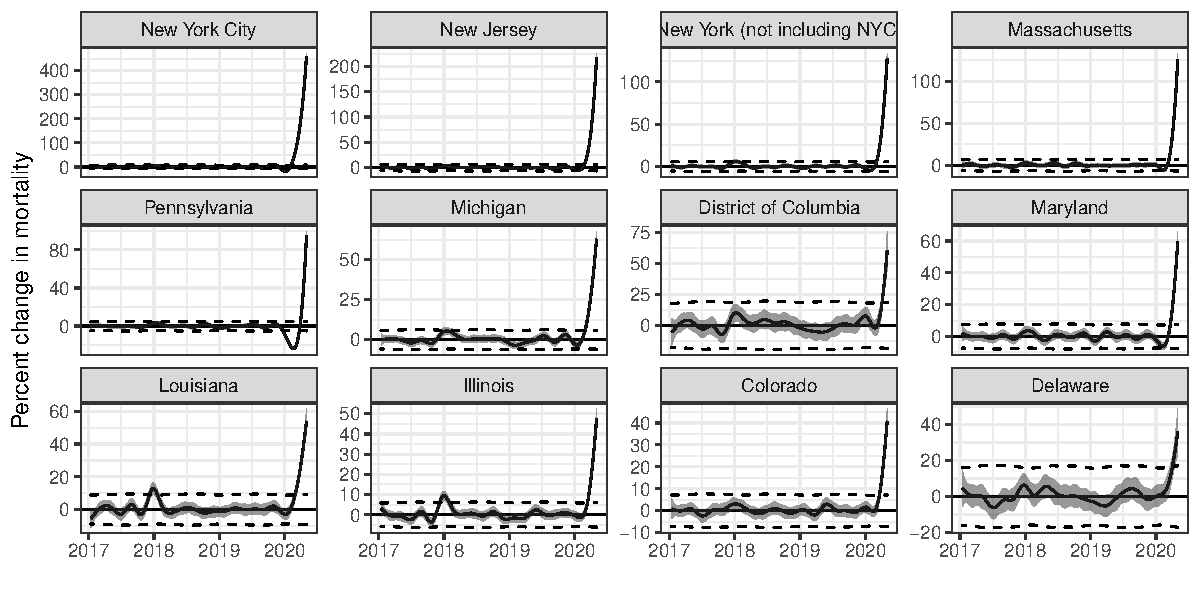
\includegraphics[width=1\linewidth]{figs/supp-figure-5.pdf} 
	\caption{Estimated event effects as percent increase over expected mortality for the top 12 jurisdictions in the United States most affected by the COVID-19 pandemic.}
	\label{supp-fig:covid19-states}
\end{suppfigure}

% Supp figure 6: Respiratory diseases mortality index
\begin{suppfigure}[ht]
	\centering
	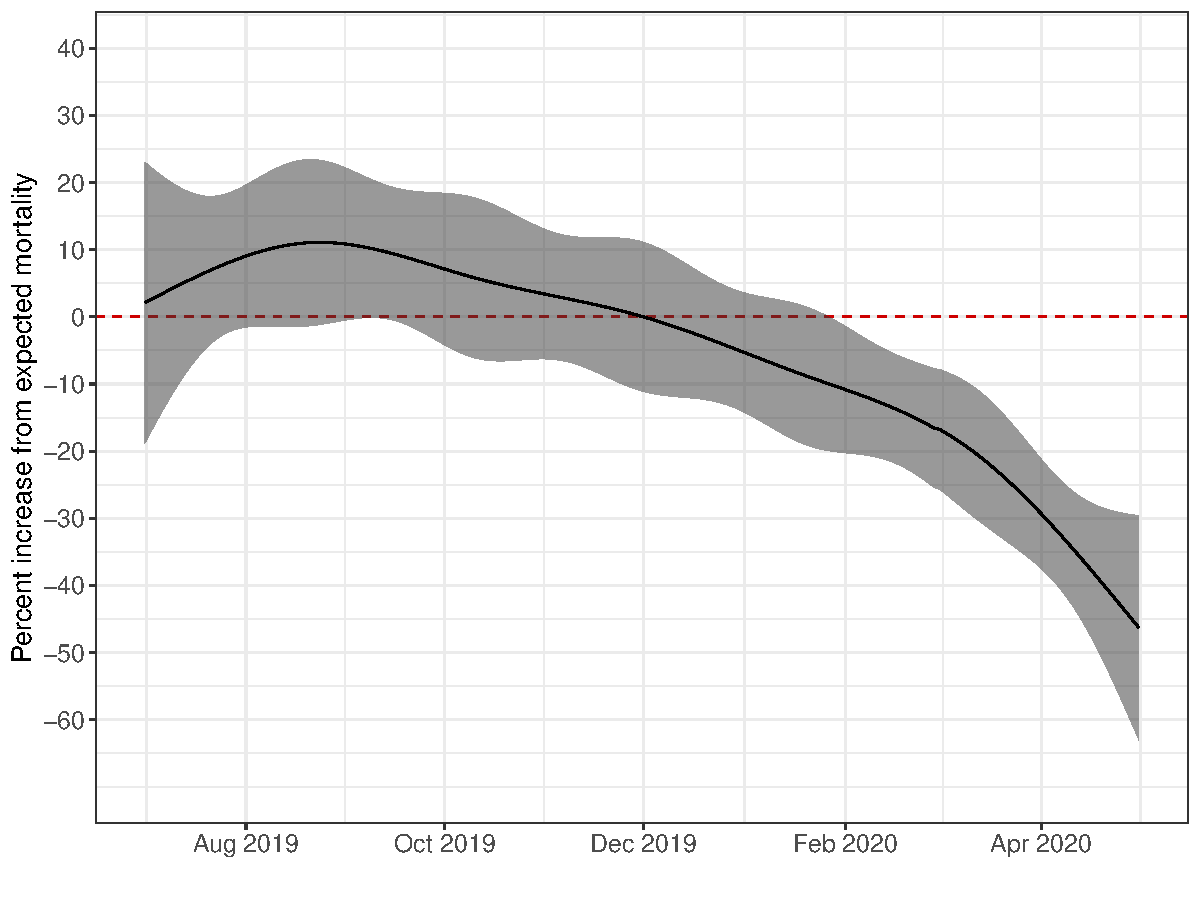
\includegraphics[width=1\linewidth]{figs/supp-figure-6.pdf} 
	\caption{Respiratory diseases mortality index. Estimated percent change in proportion of mortality, $\hat{f}(t)$, caused by respiratory diseases. The shaded area represents a 95\% confidence interval for $\hat{f}(t)$. Respiratory diseases were defined as all ICD 10 codes between J00 and J99.}
	\label{supp-fig:respiratory-index-pr}
\end{suppfigure}

% Supp figure 7: Population displacement in Puerto Rico
\begin{suppfigure}[ht]
	\centering
	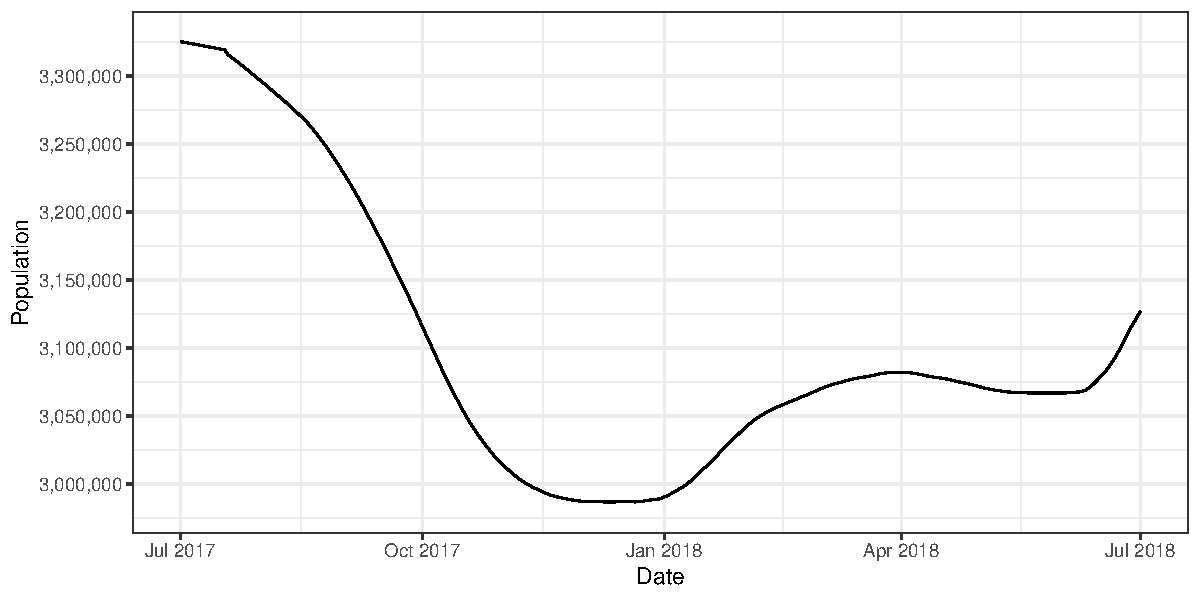
\includegraphics[width=1\linewidth]{figs/supp-figure-7.pdf} 
	\caption{Estimated population displacement in Puerto Rico after Hurricane Mar\'ia.}
	\label{supp-fig:pop-displacement-pr}
\end{suppfigure}

% Supp figure 8: Counterfactual considerations
\begin{suppfigure}[ht]
	\begin{tabular}{lll}
	A&B\\
	\begin{subfigure}[t]{0.49\linewidth}
		\centering
		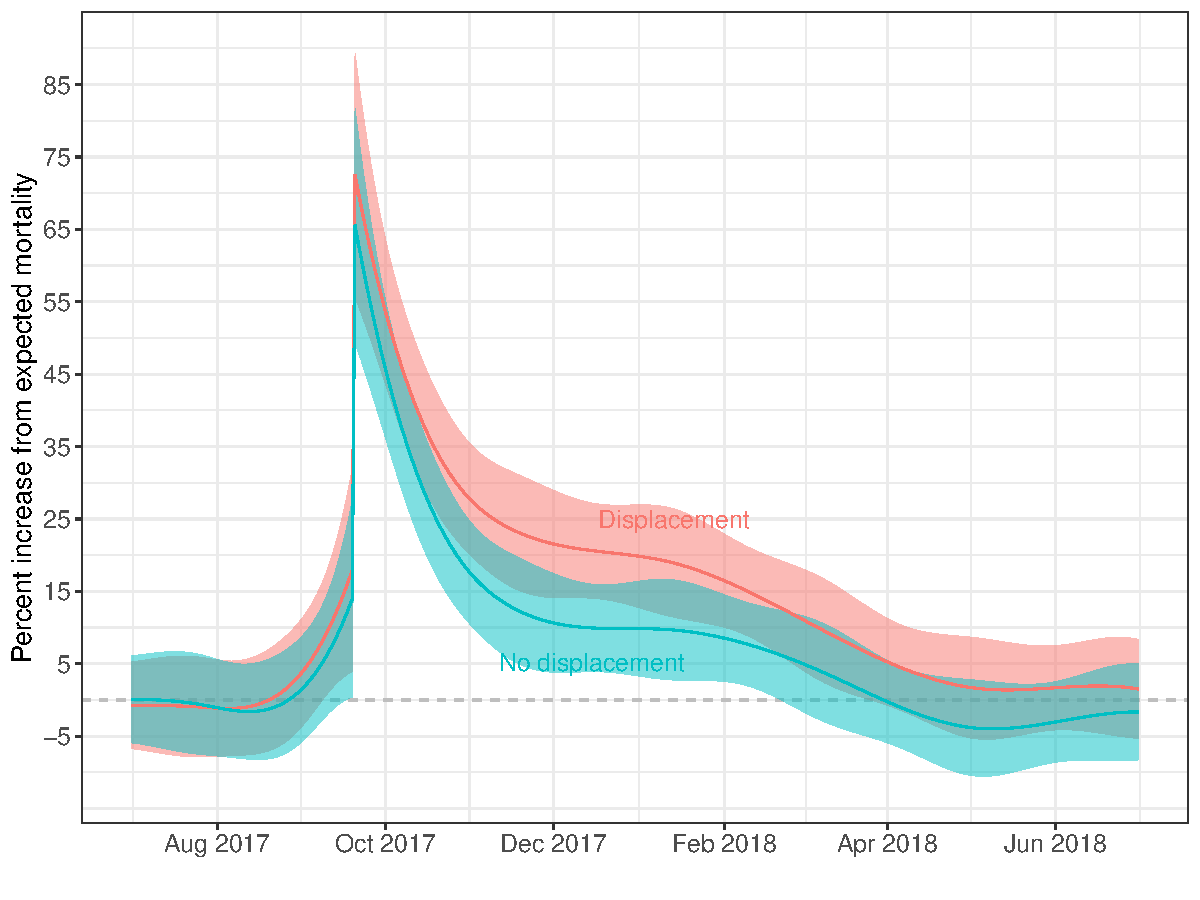
\includegraphics[width=1\linewidth]{figs/supp-figure-8a.pdf} 
	\end{subfigure}&
	\begin{subfigure}[t]{0.49\linewidth}
		\centering
		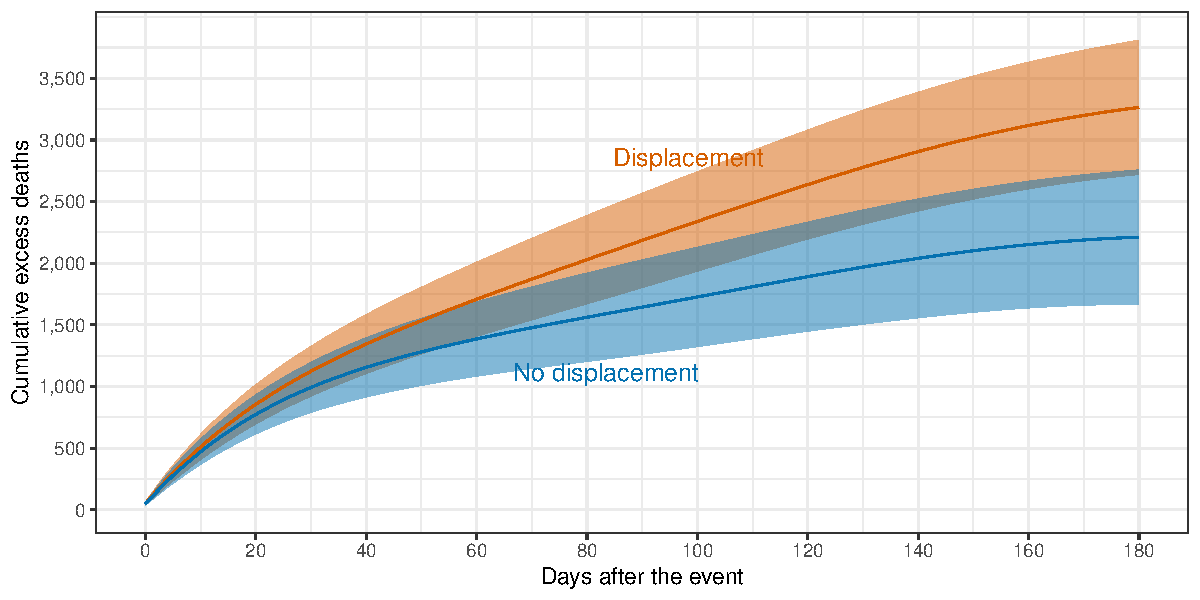
\includegraphics[width=1\linewidth]{figs/supp-figure-8b.pdf}
	\end{subfigure}&\\
    \end{tabular}
    \caption{Counterfactual considerations}
    \label{supp-fig:counterfactual-considerations}
\end{suppfigure}

% Supp figure 9: Simulation study
\begin{suppfigure}[ht]
	\begin{tabular}{lll}
	A&B&C\\
	\begin{subfigure}[t]{0.30\linewidth}
		\centering
		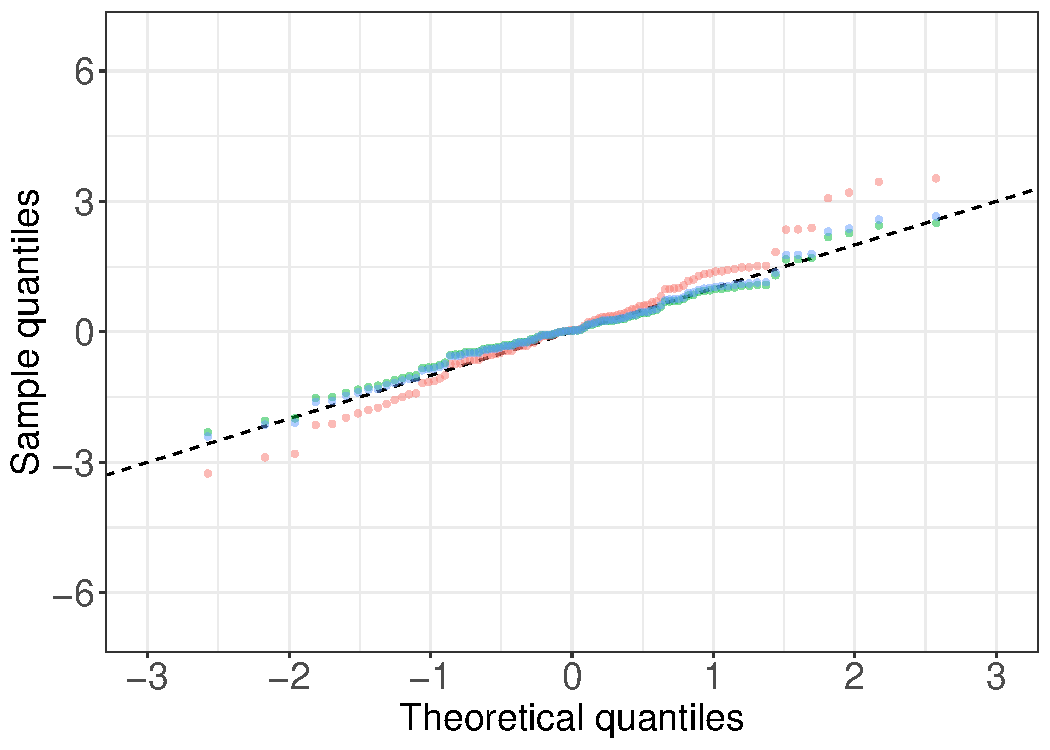
\includegraphics[width=1\linewidth]{figs/supp-figure-9a.pdf} 
	\end{subfigure}&
	\begin{subfigure}[t]{0.30\linewidth}
		\centering
		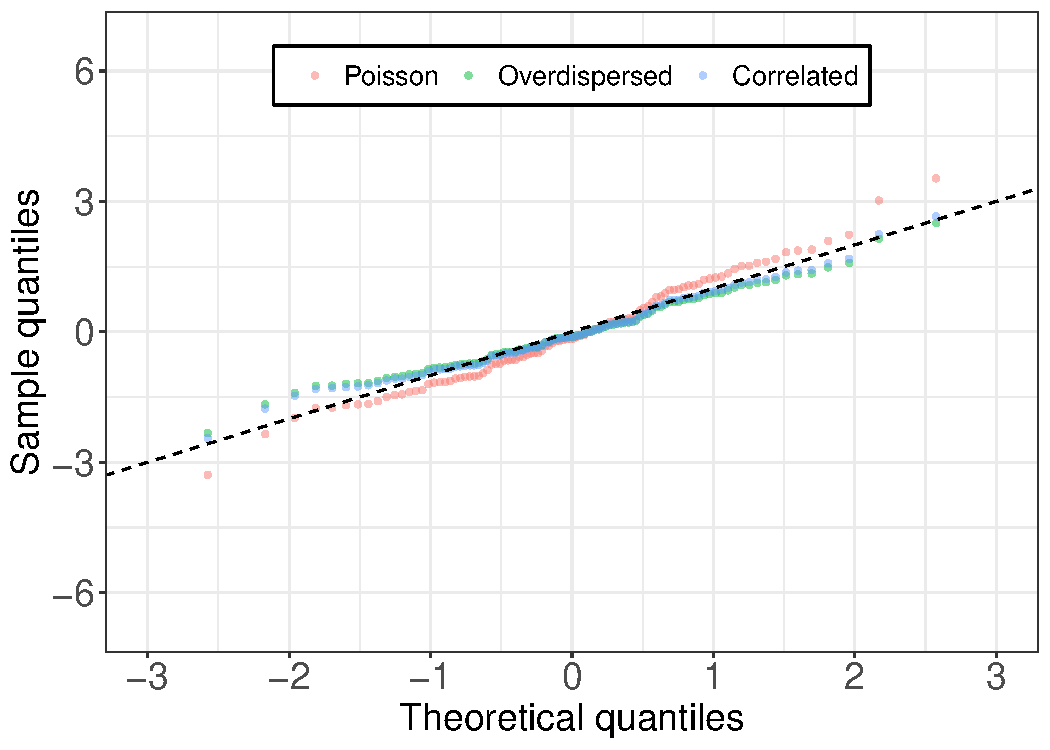
\includegraphics[width=1\linewidth]{figs/supp-figure-9b.pdf}
	\end{subfigure}&
	\begin{subfigure}[t]{0.30\linewidth}
		\centering
		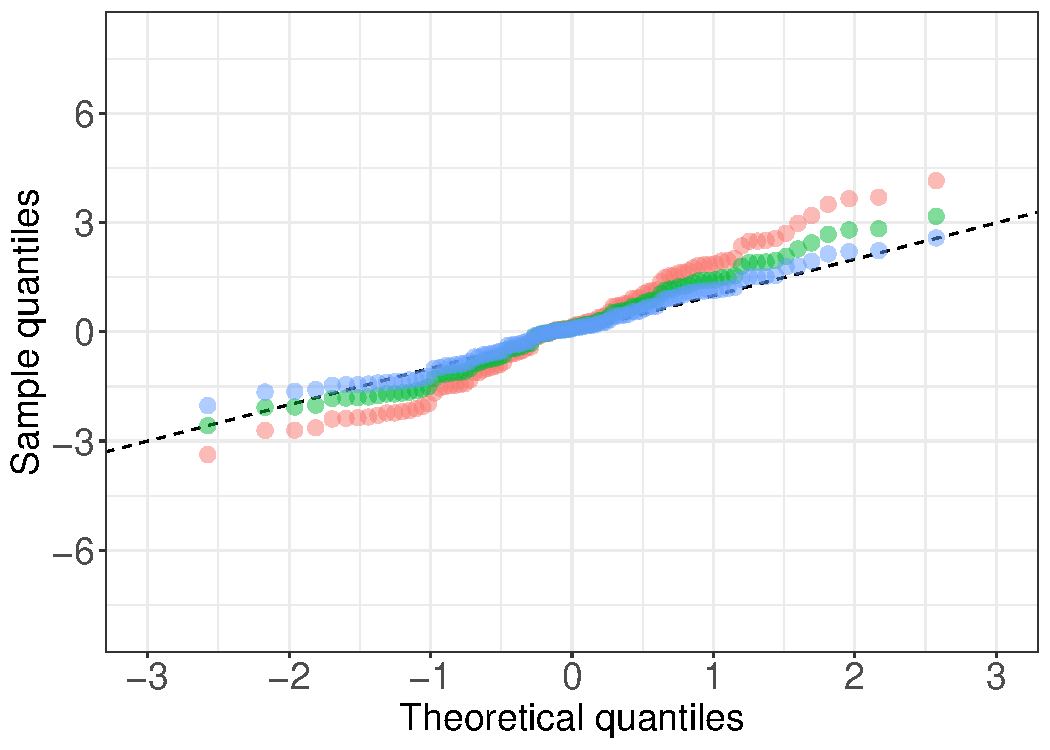
\includegraphics[width=1\linewidth]{figs/supp-figure-9c.pdf}
	\end{subfigure}\\
	D&E&F\\
	\begin{subfigure}[t]{0.30\linewidth}
		\centering
		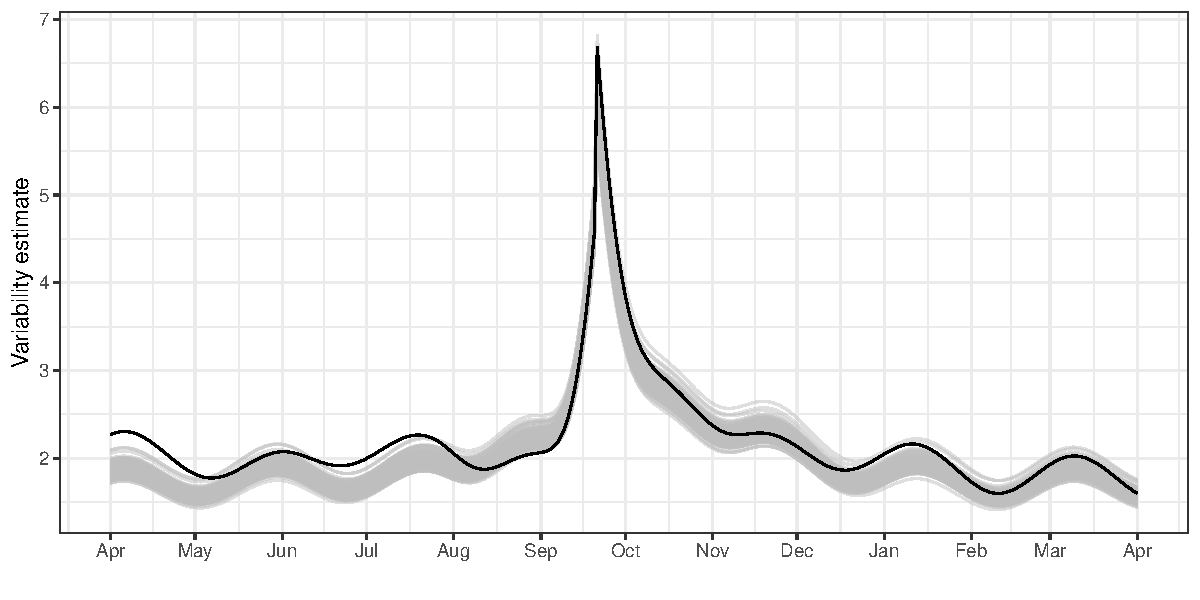
\includegraphics[width=1\linewidth]{figs/supp-figure-9d.pdf} 
	\end{subfigure}&
	\begin{subfigure}[t]{0.30\linewidth}
		\centering
		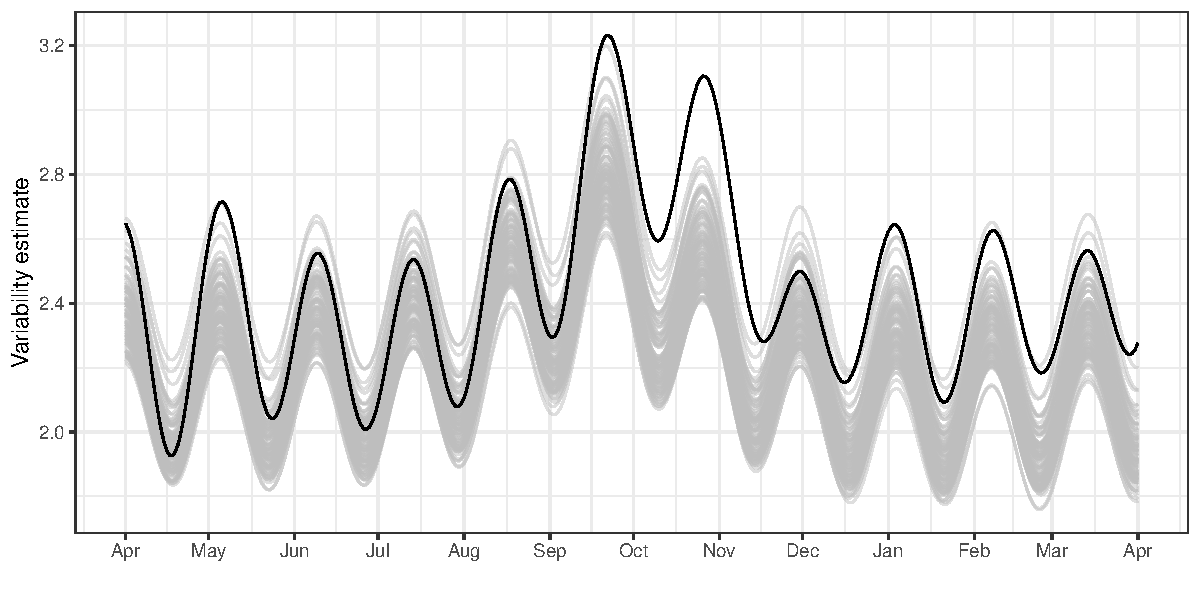
\includegraphics[width=1\linewidth]{figs/supp-figure-9e.pdf}
	\end{subfigure}&
	\begin{subfigure}[t]{0.30\linewidth}
		\centering
		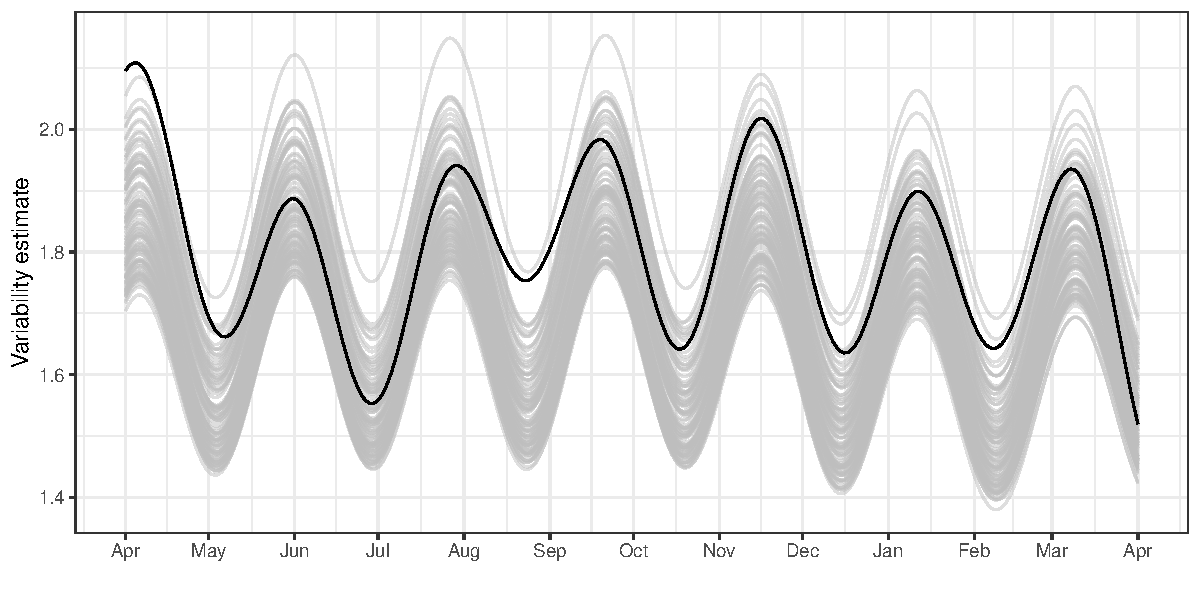
\includegraphics[width=1\linewidth]{figs/supp-figure-9f.pdf}
	\end{subfigure}\\	
    \end{tabular}
    \caption{Simulation study}
    \label{fig:simulation}
\end{suppfigure}

\end{document}

